% ============================================================================
%  PQID — A Post-Quantum Identifier for the Late 2020s and Beyond
%  Whitepaper, version 1
%
%  Build:  make
%          (or: pdflatex main && bibtex main && pdflatex main && pdflatex main)
% ============================================================================
\documentclass[11pt,letterpaper]{article}

% ---- Geometry / typography ----
\usepackage[margin=1in,top=1in,bottom=1.1in]{geometry}
\usepackage[utf8]{inputenc}
\usepackage[T1]{fontenc}
\usepackage{lmodern}            % crisp Latin Modern fonts
\usepackage{microtype}          % subtle letter-spacing improvements
\usepackage{parskip}            % no paragraph indent, vertical space between paras
\usepackage{setspace}
\setstretch{1.05}

% ---- Math, code, color, tables, figures, citations ----
\usepackage{amsmath,amssymb}
\usepackage{xcolor}
\usepackage{listings}
\usepackage{booktabs}
\usepackage{array}
\usepackage{longtable}
\usepackage{tabularx}
\usepackage{tcolorbox}
\tcbuselibrary{breakable,skins}
\usepackage{tikz}
\usetikzlibrary{positioning,shapes,arrows.meta,decorations.pathreplacing,calc}
\usepackage[round,authoryear]{natbib}
\bibliographystyle{abbrvnat}

% ---- Hyperlinks ----
\usepackage[colorlinks=true,linkcolor=blue!50!black,citecolor=blue!50!black,urlcolor=blue!50!black,bookmarksopen=true]{hyperref}
\usepackage[nameinlink]{cleveref}

% ---- Headers / footers ----
\usepackage{fancyhdr}
\pagestyle{fancy}
\fancyhf{}
\fancyhead[L]{\small\textsl{PQID Whitepaper}}
\fancyhead[R]{\small\textsl{\leftmark}}
\fancyfoot[C]{\small \thepage}
\renewcommand{\headrulewidth}{0.4pt}

% ---- Listings (code) ----
\definecolor{codebg}{rgb}{0.97,0.97,0.97}
\definecolor{codecomment}{rgb}{0.30,0.50,0.30}
\definecolor{codekw}{rgb}{0.10,0.30,0.70}
\definecolor{codestr}{rgb}{0.65,0.20,0.20}
\definecolor{codenum}{rgb}{0.50,0.50,0.50}
\lstdefinestyle{pqidcode}{
  backgroundcolor=\color{codebg},
  basicstyle=\ttfamily\footnotesize,
  keywordstyle=\color{codekw}\bfseries,
  commentstyle=\color{codecomment}\itshape,
  stringstyle=\color{codestr},
  numberstyle=\tiny\color{codenum},
  numbers=left,
  numbersep=8pt,
  xleftmargin=15pt,
  framesep=4pt,
  frame=single,
  framerule=0.4pt,
  rulecolor=\color{black!30},
  showspaces=false,
  showstringspaces=false,
  breaklines=true,
  breakatwhitespace=true,
  tabsize=2,
  captionpos=b,
}
\lstset{style=pqidcode}
\lstdefinelanguage{Pseudocode}{
  morekeywords={if,else,then,return,for,while,procedure,function,end,true,false,when,or,and,not,case,default,is,error},
  morecomment=[l]{//},
  morecomment=[l]{\#},
  sensitive=true,
}

% ---- Callouts (info / warning) ----
\newtcolorbox{calloutinfo}[1][]{
  enhanced, breakable, colback=blue!4, colframe=blue!50!black, fonttitle=\bfseries,
  left=8pt, right=8pt, top=4pt, bottom=4pt, title=#1
}
\newtcolorbox{calloutwarning}[1][]{
  enhanced, breakable, colback=orange!6, colframe=orange!70!black, fonttitle=\bfseries,
  left=8pt, right=8pt, top=4pt, bottom=4pt, title=#1
}

% ---- Section formatting ----
\usepackage{titlesec}
\titleformat{\section}{\Large\bfseries}{\thesection}{1em}{}
\titleformat{\subsection}{\large\bfseries}{\thesubsection}{1em}{}
\titleformat{\subsubsection}{\normalsize\bfseries}{\thesubsubsection}{1em}{}
\titlespacing{\section}{0pt}{18pt}{8pt}
\titlespacing{\subsection}{0pt}{14pt}{6pt}

% ---- Custom commands ----
\newcommand{\pqid}{\textsf{PQID}}
\newcommand{\code}[1]{\texttt{#1}}

% ============================================================================
%  Document
% ============================================================================
\begin{document}

% ---- Title page ----
% Auto-generated at build time. Do not edit.
\newcommand{\buildDate}{May 20, 2026}
\newcommand{\buildTime}{09:28 UTC}
  % generated at build time: \buildDate, \buildTime
\begin{titlepage}
  \centering
  \vspace*{2.5cm}
  {\Huge\bfseries PQID\par}
  \vspace{0.6cm}
  {\Large A Post-Quantum Identifier for the\\Late 2020s and Beyond\par}
  \vspace{2cm}
  {\large\itshape Whitepaper, Version 1\par}
  \vspace{2cm}
  \begin{tcolorbox}[colback=gray!5,colframe=black!30,width=0.7\textwidth]
    \centering\small
    \textbf{Build date:} \buildDate\\[0.3em]
    \textbf{Build time:} \buildTime\\[0.3em]
    \textbf{Source:} \texttt{pqid/latex/main.tex}
  \end{tcolorbox}
  \vfill
  {\small This document is the canonical reference for PQID v1.\par}
  \vspace{0.5cm}
\end{titlepage}

\setcounter{tocdepth}{2}
\tableofcontents
\newpage

% ---- Sections (one file per part) ----
% ============================================================================
%  TL;DR
% ============================================================================
\section*{TL;DR}
\addcontentsline{toc}{section}{TL;DR}

\textsf{PQID} is a 41-byte, lexicographically-sortable identifier designed to be useful for the next thirty years of distributed systems. It pairs a 48-bit millisecond timestamp with 256 bits of cryptographically-strong randomness --- the smallest random field that retains 128 bits of effective security under Grover's quantum search algorithm \citep{grover1996}. A version byte and a 16-bit per-millisecond counter sit between them. Two variants of the format share the same wire layout: \textbf{Standard} (variant \code{0x01}) for centralized generation against a wall clock, and \textbf{Hybrid Logical Clock} (variant \code{0x02}) for distributed systems where causal ordering across nodes matters \citep{kulkarni2014hlc}.

PQID encodes to \textbf{55 characters} of canonical Base64URL \citep{rfc4648} or \textbf{66 characters} of human-typable Crockford Base32 \citep{crockford}. Both encodings round-trip to identical 41-byte binary values, and binary sort and Crockford ASCII sort both reflect generation time. (Canonical Base64URL preserves byte order only when compared as bytes --- its alphabet ordering does not match ASCII codepoint order, so consumers that need a textual column to sort by time should use Crockford or sort the underlying bytes.) The 55-character Base64URL form fits comfortably in URL paths, JSON, headers, and database primary-key columns; the Crockford form is meant for human transcription, log lines, CLI tools, and any column where lexicographic text sort must reflect generation time.

The format runs at over \textbf{2.1 million IDs/second per thread} in C, C++, Rust, and Java on a 2.10\,GHz x86-64 core, and at over 4.6\,M IDs/sec in Go. The bottleneck across every implementation is the OS CSPRNG, not PQID's own logic. Time-sortedness across consecutive IDs is 100\% by construction, matching ULID \citep{ulid} and beating UUIDv4 \citep{rfc4122}, UUIDv7 \citep{rfc9562}, and KSUID \citep{ksuid}.

This document is the canonical reference for PQID v1: the wire format, the rationale for every numeric choice, when to use each variant, how to implement generators correctly, the security model, the distributed-systems model, detailed comparisons against UUIDv4, UUIDv7, ULID, KSUID, and Snowflake, and \textbf{eight reference implementations} (Python, Go, Rust, TypeScript, C, C++, Java, and a CPython extension) with verified benchmark data.

\begin{calloutinfo}[The million-node regime]
At the scales now emerging in frontier-AI training clusters and globally-distributed inference fleets, PQID is the only published format whose collision math, coordination model, causal-ordering semantics, and post-quantum margins all hold simultaneously. UUIDv4 fails on collision math (the 122-bit random field is undersized for trillions of identifiers per training run). UUIDv7 fails on intra-millisecond sort guarantees (RFC 9562 §6.2 permits implementations that randomize within a ms) and on causal ordering across geographically-distributed nodes. ULID and KSUID fail on entropy. Snowflake \citep{snowflake} fails on coordination requirements. Part \ref{sec:ai-scale} makes this case in detail.
\end{calloutinfo}


% ============================================================================
%  Part I: Why a New Identifier
% ============================================================================
\section{Why a New Identifier}
\label{sec:why}

Every identifier format reflects the constraints and assumptions of the moment it was designed. The decisions baked into UUIDv4 \citep{rfc4122} in 2005 --- 128 bits total, 122 bits of entropy, no time component, no ordering --- made sense when distributed databases were rare, quantum computers were a footnote, and ``unique'' meant ``unique in this rack.'' Twenty years later, the constraints have shifted enough that even the carefully-chosen successors to UUIDv4 (UUIDv7 \citep{rfc9562}, ULID \citep{ulid}, KSUID \citep{ksuid}) leave gaps. PQID is an attempt to fill the remaining gaps in a single, coherent format --- not by adding features, but by making slightly different choices on three numbers: the size of the random field, the granularity of the timestamp, and the semantics of the version byte.

\subsection{Quantum search has changed the entropy budget}

Grover's algorithm \citep{grover1996} gives a quantum computer a quadratic speedup over classical search: finding a single matching value among $2^n$ candidates takes approximately $2^{n/2}$ quantum operations. For an identifier whose security model rests on the difficulty of guessing a specific value (a \emph{targeted second preimage}), that means an $n$-bit random field gives only $n/2$ bits of effective post-quantum security. UUIDv4's 122 bits give 61. UUIDv7's 74 give 37. ULID's 80 give 40. KSUID's 128 give 64. PQID's 256 give 128 --- the level NIST has designated as adequate for symmetric primitives through 2030 and beyond \citep{nist80057}, and the level ML-DSA-44 \citep{fips204} and ML-KEM-512 \citep{fips203} are calibrated to. Choosing less for a new identifier means accepting that the identifier becomes the weakest cryptographic component of any system that combines it with AES-128 \citep{fips197} or stronger. Part \ref{sec:security} works through the math (Grover, BHT \citep{bht1998}, the classical and quantum birthday bounds) in detail.

\subsection{Time-sortability is a feature, not a side effect}

Random identifiers like UUIDv4 are catastrophic for B-tree indexes. Each new insert lands at a random point in the tree, causing scattered page writes, poor cache behavior, and eventually fragmentation that degrades read performance. The fix is well-understood: prefix the identifier with a timestamp so consecutive inserts land near each other. ULID, KSUID, and UUIDv7 all do this. PQID does too.

But there's a subtlety. ULID and KSUID expose lexicographic byte ordering as a first-class property: sorting their bytes (or, in ULID's case, their Crockford-encoded strings) yields time-ordering. UUIDv7's RFC permits implementations that randomize within a millisecond in ways that break this property; the spec only guarantees ordering \emph{between} milliseconds, not \emph{within} them. PQID guarantees both. Within a single millisecond, a per-generator counter makes consecutive IDs strictly increasing; across milliseconds, the timestamp dominates. The result is 100\% time-sortedness across consecutive IDs from a single generator (binary order, and ASCII order in the Crockford encoding), measured against 10{,}000 consecutive IDs in the benchmark suite and against 100{,}000 unique IDs in the uniqueness test.

\subsection{Distributed systems need first-class causal ordering}

The Standard variant uses a wall-clock timestamp. That works fine when a single machine is producing IDs --- the local clock is the source of truth and consumers that care about ordering get what they expect. It works less well when many machines are producing IDs and clocks disagree by tens of milliseconds.

The HLC variant solves this. A Hybrid Logical Clock \citep{kulkarni2014hlc} combines physical time with a logical counter. An HLC reading is always at least the maximum of the local wall clock and any HLC value the node has observed from a peer; the counter increments whenever logical time fails to advance. The result is a clock that stays close to physical time, always moves forward, and preserves causal ordering across nodes that exchange HLC values in their messages.

PQID's HLC variant exposes that machinery as a first-class identifier shape. The wire format is identical to the Standard variant; the only difference is the variant byte (\code{0x02} instead of \code{0x01}) and the semantic interpretation of the timestamp (logical, not physical, with a 60-second drift bound). A consumer that doesn't care about variant semantics can sort PQIDs as opaque bytes and get correct ordering across both variants in the same stream.

\subsection{The cost: bytes}

PQID's distinguishing properties are the 256-bit random field --- the only format with comfortable post-quantum margins --- and the dual-variant design that makes the same wire format usable for both centralized and distributed generation. The cost is byte-count: at 41 bytes binary or 55 characters Base64URL, PQID is roughly $2.5\times$ the size of UUIDv4. Part \ref{sec:compare} works through the format-by-format tradeoffs; Part \ref{sec:when} maps them onto specific use cases.


% ============================================================================
%  Part II: PQID Specification (normative)
% ============================================================================
\section{PQID Specification}
\label{sec:spec}

This part is the normative reference. Implementations that conform to this specification produce and consume identifiers with the byte layout, semantics, and encoding rules described below. Where this document uses RFC 2119 keywords (MUST, SHOULD, MAY), they carry the standard meanings.

\subsection{Wire format}

A PQID is exactly 41 bytes (328 bits), structured as four contiguous fields:

\begin{center}
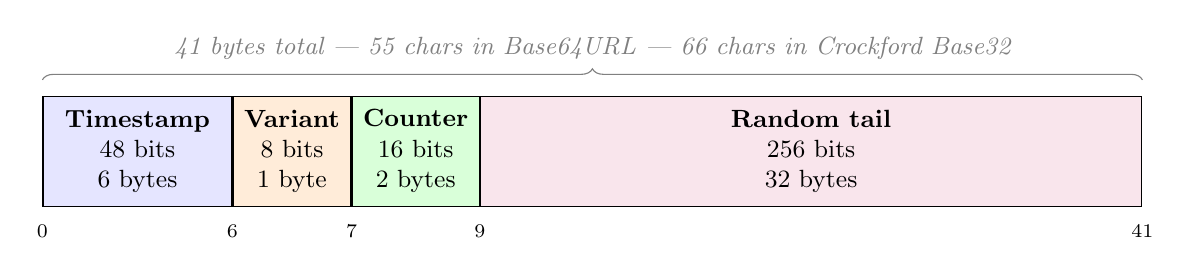
\begin{tikzpicture}[
    field/.style={draw,minimum height=14mm,inner sep=4pt,align=center,font=\small},
    label/.style={font=\scriptsize\itshape,gray},
    bytelabel/.style={font=\scriptsize,below=1mm}
  ]
  % Field rectangles (widths roughly proportional to bit widths)
  \node[field, fill=blue!10,    minimum width=24mm] (ts)  at (0,0)    {\textbf{Timestamp}\\48 bits\\6 bytes};
  \node[field, fill=orange!15,  minimum width=10mm, right=0pt of ts]  (ver) {\textbf{Variant}\\8 bits\\1 byte};
  \node[field, fill=green!15,   minimum width=14mm, right=0pt of ver] (ctr) {\textbf{Counter}\\16 bits\\2 bytes};
  \node[field, fill=purple!10,  minimum width=84mm, right=0pt of ctr] (rnd) {\textbf{Random tail}\\256 bits\\32 bytes};

  % Byte offset markers
  \node[bytelabel] at (ts.south west) {0};
  \node[bytelabel] at (ts.south east) {6};
  \node[bytelabel] at (ver.south east) {7};
  \node[bytelabel] at (ctr.south east) {9};
  \node[bytelabel] at (rnd.south east) {41};

  % Total span brace
  \draw[decorate,decoration={brace,amplitude=4pt}, gray]
    ($(ts.north west)+(0,2mm)$) -- ($(rnd.north east)+(0,2mm)$)
    node[midway,above=4pt,font=\small\itshape] {41 bytes total --- 55 chars in Base64URL --- 66 chars in Crockford Base32};
\end{tikzpicture}
\end{center}

\textbf{Field semantics}:
\begin{description}
  \item[Timestamp (offsets 0--5).] Big-endian unsigned 48-bit integer, milliseconds since the Unix epoch (1970-01-01T00:00:00Z). The 48-bit field provides $2^{48}$ ms $\approx$ 8{,}919 years of forward range, sufficient through the year 10889.
  \item[Variant (offset 6).] Single byte.
    \begin{itemize}
      \item \code{0x01} = Standard (wall-clock).
      \item \code{0x02} = HLC (Hybrid Logical Clock).
      \item \code{0x00} and \code{0xFF} are \textbf{permanently reserved}: they MUST be rejected by conformant decoders and MUST NOT be assigned in any future revision of this specification. These two values are reserved defensively so that PQID buffers cannot be confused with zero-filled or all-ones uninitialized memory.
      \item \code{0x03}--\code{0xFE} are reserved for future variants. Conformant decoders MUST reject them with an unknown-variant error until they are assigned by a future revision of this specification.
    \end{itemize}
  \item[Counter (offsets 7--8).] Big-endian unsigned 16-bit integer. For Standard, the counter is incremented within a single millisecond by a small random step (1--16); for HLC, it is the HLC logical counter.
  \item[Random tail (offsets 9--40).] 32 bytes from a cryptographically-strong random source. The full 256 bits provide $2^{128}$ effective post-quantum security against second-preimage attacks.
\end{description}

\subsection{Standard variant generation (variant \code{0x01})}

The Standard generation algorithm assumes a wall-clock time source that returns milliseconds since the Unix epoch. It maintains two pieces of per-generator state: \code{last\_ts} (initially 0) and \code{counter} (initially 0).

\begin{lstlisting}[language=Pseudocode,caption={Standard PQID generation},label={lst:gen-std}]
procedure new_standard():
    rnd[0..32]  <-  csprng()           # 33 bytes total
    ts          <-  now_ms()
    if ts < last_ts:                   # clamp on regression
        ts  <-  last_ts
    if ts == last_ts:                  # same ms as previous ID
        step    <-  1 + (rnd[0] & 0x0F)    # random step in [1, 16]
        next    <-  counter + step
        if next > 0xFFFF:              # counter exhausted, spin
            while now_ms() <= last_ts: pass
            ts       <-  now_ms()
            counter  <-  rnd[0]        # reseed at small value
        else:
            counter  <-  next
    else:                              # new ms
        counter  <-  rnd[0]            # randomized initial offset
    last_ts <-  ts
    return  be48(ts) || 0x01 || be16(counter) || rnd[1..32]
\end{lstlisting}

The random step (rather than a fixed +1 increment) is a deliberate choice. It provides modest unlinkability of consecutive IDs from a single generator while preserving strict monotonicity (the step is always at least 1, so consecutive IDs always increase).

\subsection{Optional defensive helper: \code{validate\_min\_timestamp}}
\label{sec:min-timestamp}

Implementations SHOULD expose a non-normative helper that returns true iff a decoded PQID's timestamp is at or after a project epoch \code{MIN\_TIMESTAMP\_MS}. The reference value is \code{1{,}700{,}000{,}000{,}000} ms ($\approx$ 2023-11-14), chosen as the earliest plausible timestamp any PQID-aware deployment will ever emit.

This helper is \textbf{not part of the wire contract}. Standard decoders MUST continue to accept all timestamps in $[0, 2^{48} - 1]$ as required by the field semantics in §\ref{sec:why}. The helper exists for callers who want to cheaply reject obvious mis-parses — a 41-byte buffer that decodes to timestamp~0 has either come from zeroed memory, a wrong-offset read, or a buggy producer. Rejecting such inputs at boundary entry points is a defense-in-depth measure, not a conformance requirement.

\subsection{CSPRNG requirements}
\label{sec:csprng}

The 256-bit random tail is the only field carrying the post-quantum security claim. Conformant implementations MUST therefore use an operating-system-provided cryptographically-strong pseudorandom number generator. The following normative rules apply:

\begin{description}
  \item[Source.] Generators MUST draw the random tail from one of: \code{getrandom(2)} on Linux 3.17+, \code{arc4random\_buf} or \code{getentropy(3)} on the BSDs and macOS, \code{BCryptGenRandom} on Windows, the language-level wrappers around these (\code{os.urandom}, \code{crypto/rand.Read}, \code{getrandom::fill}, \code{crypto.getRandomValues}, \code{SecureRandom}), or — as a last-resort portable fallback — \code{/dev/urandom}. Generators MUST NOT use a non-cryptographic userspace PRNG (Mersenne Twister, Xoshiro, \code{rand}, etc.) under any circumstance.
  \item[Failure.] If the CSPRNG returns an error or refuses to produce 32 bytes, the generator MUST surface the error to the caller and MUST NOT emit a PQID. There is no fallback path.
  \item[Partial reads.] Partial reads (an underlying \code{read()} or \code{getrandom()} returning fewer than 32 bytes) MUST be retried until either 32 bytes are obtained or an unrecoverable error is returned.
  \item[Independence.] Each PQID's random tail MUST be drawn independently. A generator MAY combine the 32-byte tail with a small additional read (1--2 bytes) used for the counter step in the same syscall as an optimization; this is unrelated to the cryptographic claim and does not weaken it because the OS CSPRNG output is uniform.
\end{description}

\noindent A test vector cannot directly verify entropy quality, but conformance reviewers SHOULD spot-check each implementation's call site against this list. The current implementations call: \code{os.urandom} (Python), \code{getrandom}/\code{getentropy} (C/C++), \code{crypto/rand.Read} (Go), \code{getrandom::fill} (Rust), \code{crypto.getRandomValues}/\code{randomFillSync} (TypeScript), \code{SecureRandom} (Java), and the underlying C reference (CPython extension).

\subsection{HLC variant generation (variant \code{0x02})}

The HLC generator maintains \code{l} (logical time, ms-grained) and \code{c} (logical counter). On every generation, it consults both the local physical clock and any peer HLC observation.

The contract uses two thresholds, distinct in purpose:

\begin{description}
  \item[Hard outer bound $\Delta_{\max} = 60{,}000$ ms (normative).] Conformant generators MUST reject observations whose logical time exceeds the local physical clock by more than $\Delta_{\max}$. Implementations MUST expose this constant under the name \code{HLC\_MAX\_DRIFT\_MS} (or the language's idiomatic equivalent). $\Delta_{\max}$ is part of the wire contract: a 60-second peer-ahead-of-local observation that one implementation accepts and another rejects is an interoperability bug.
  \item[Soft alarm threshold $\Delta_{\text{alarm}}$ (configurable, default 1{,}000 ms).] Implementations SHOULD emit a log, metric, or alarm when an observation exceeds $\Delta_{\text{alarm}}$, even if it is still below $\Delta_{\max}$. The default of 1 second captures the operational reality that well-disciplined hosts (NTP, chrony, AWS Time Sync, GCP) maintain sub-100~ms drift; a peer 1~s ahead almost certainly indicates a clock-discipline or NTP-outage problem that an operator should know about, even though the wire format still accepts it. $\Delta_{\text{alarm}}$ is NOT part of the wire contract.
\end{description}

\noindent The rationale for $\Delta_{\max} = 60$~s: large enough to absorb a brief NTP outage, container time injection, or VM live-migration without breaking valid traffic; small enough that a maliciously advanced peer cannot stamp identifiers a year into the future. The HLC literature (Kulkarni et al.~2014, \S3) explicitly leaves the bound to operators; the CockroachDB and kronos operational practice in production is approximately 500~ms to 1~s. We pick 60~s for the hard bound because the wire-format invariant should tolerate the worst plausible operational event without changing, and we pick 1~s as the default alarm because that's where well-run systems already live.

\begin{lstlisting}[language=Pseudocode,caption={HLC PQID generation (with optional peer observation)},label={lst:gen-hlc}]
procedure new_hlc(observe = none):
    rnd[0..31] <- csprng()             # 32 bytes
    pt         <- now_ms()             # physical time
    l_old, c_old <- l, c
    if observe is not none:
        l_msg, c_msg <- observe
        if (l_msg > pt) and ((l_msg - pt) > MAX_DRIFT_MS):
            error  HLC_drift_exceeded
        l_new <- max(l_old, l_msg, pt)
        case:
            l_new == l_old == l_msg:  c_new <- max(c_old, c_msg) + 1
            l_new == l_old:           c_new <- c_old + 1
            l_new == l_msg:           c_new <- c_msg + 1
            default:                  c_new <- 0
    else:
        l_new <- max(l_old, pt)
        c_new <- (c_old + 1) when l_new == l_old, else 0
    if c_new > 0xFFFF: l_new += 1; c_new <- 0
    l, c <- l_new, c_new
    return  be48(l_new) || 0x02 || be16(c_new) || rnd
\end{lstlisting}

\subsection{Text encodings}

PQID defines two text encodings. Both round-trip cleanly to the same 41-byte binary form and neither uses padding. They differ in their behavior under string sort: Crockford Base32 \citep{crockford} is ASCII-sort-preserving (sorting the strings as text gives generation-time order), while canonical Base64URL is sort-preserving only when its bytes are compared, not when its text is compared as ASCII. The reason is that the RFC 4648 §5 alphabet \citep{rfc4648} (\code{A--Z}, \code{a--z}, \code{0--9}, \code{-}, \code{\_}) maps alphabet values 0..63 to ASCII codepoints that are not monotonic --- \code{A--Z} (65..90), \code{a--z} (97..122), \code{0--9} (48..57), \code{-} (45), \code{\_} (95) interleave, so a string-level ASCII sort produces an order different from the underlying byte order. Crockford's alphabet (\code{0--9} then \code{A--Z} minus \code{I/L/O/U}) is monotonic in ASCII and so its strings sort identically to their decoded bytes. Choose accordingly: machine-to-machine paths use Base64URL and sort the bytes (or simply preserve insertion order); human-facing or text-sorted columns use Crockford.

\subsubsection{Canonical: Base64URL (55 characters)}

RFC 4648 Section 5 (``Base 64 Encoding with URL and Filename Safe Alphabet''), no padding. Encoding 41 bytes produces $\lceil 41 \cdot 8 / 6 \rceil = 55$ characters; the final character carries 4 bits of value plus 2 bits of zero padding. The alphabet is \code{A-Z}, \code{a-z}, \code{0-9}, \code{-}, \code{\_}. Decoders MUST reject inputs whose final character carries non-zero padding bits.

\subsubsection{Human-typable: Crockford Base32 (66 characters)}

Crockford's alphabet (\code{0123456789ABCDEFGHJKMNPQRSTVWXYZ}) and its case-insensitive decoding (with the I/L→1 and O→0 confusables canonicalized) make this encoding suitable for human transcription. Encoding 41 bytes produces $\lceil 41 \cdot 8 / 5 \rceil = 66$ characters; the final character carries 3 bits of value plus 2 bits of zero padding.

The Crockford form is intended for use cases where humans handle the identifier directly: pasted into chat messages, read aloud over phones, written on paper, or appearing in CLI tools where mixed-case is hostile. The Base64URL form is intended for everything else.


% ============================================================================
%  Part III: Why Each Choice
% ============================================================================
\section{Why Each Choice}
\label{sec:rationale}

This part walks through every numeric and structural choice in the PQID specification and explains why the choice was made. The intent is to make the reasoning transparent enough that a reader can disagree on first principles rather than wondering whether a number came out of a hat.

\subsection{Why 256 random bits?}

The 256-bit random tail is the largest single design choice in PQID. It is the reason PQID is 41 bytes rather than 16, 20, or 24. The alternative --- 128 random bits, fitting comfortably inside a 24-byte identifier --- gives 64-bit post-quantum security against birthday-bound collisions, which is plenty for almost every classical use case but uncomfortable as a long-term margin in the regime where quantum search is a credible threat. The 256-bit choice is calibrated to give 128 bits of effective post-quantum security against a targeted second-preimage attack, matching the level NIST has designated as adequate for symmetric primitives through 2030 and beyond. Part \ref{sec:security} carries the full Grover/BHT/birthday-bound derivation.

The cost is sixteen extra bytes per identifier --- the same level the cryptographic community has converged on for symmetric primitives like AES-256 \citep{fips197} and SHA-256-based \citep{fips180} hashes. In an era where average HTTP responses are kilobytes and average database row sizes are hundreds of bytes, sixteen bytes is unremarkable.

\subsection{Why a 48-bit millisecond timestamp?}

Forty-eight bits of milliseconds gives roughly 8{,}919 years of forward range. We chose this over 32 bits (which gives 49 days from epoch and would have wrapped already) and 64 bits (which gives 584 million years and would be wasteful). Forty-eight bits is the same width Snowflake \citep{snowflake} uses for its timestamp, the same width UUIDv7 \citep{rfc9562} uses, and the same width ULID \citep{ulid} uses. The cross-format consistency is convenient.

Millisecond granularity is a compromise. Microseconds (or nanoseconds) would let two consecutive IDs from a single generator fall into different timestamp buckets without needing a counter, but cross-machine clock skew is typically larger than a microsecond, so the apparent gain is illusory. Seconds would mean every server in a cluster could collide with every other server every second, and the counter would have to be much larger to recover order. Milliseconds split the difference: per-millisecond collisions across nodes are common but recoverable from the random tail; per-millisecond collisions within a single node are eliminated by the counter.

If you genuinely need finer ordering across nodes --- closer to single-microsecond --- the right tool is the HLC variant, which captures causal ordering through message exchange rather than relying on synchronized clocks. The Standard variant accepts that wall-clock granularity below a millisecond is a fiction and stops there.

\subsection{Why a single-byte variant byte rather than two formats?}

Two design choices were considered for the relationship between Standard and HLC PQIDs: separate identifier formats with separate names, or a single format with a discriminator byte. The variant-byte approach won on three grounds.

\textbf{Wire-format compatibility.} Both variants are 41 bytes, both encode and decode identically, and both are lexicographically sortable. A consumer that has no opinion about whether an identifier was generated against a wall clock or an HLC can treat all PQIDs as opaque sortable bytes; only consumers that care about the timestamp's semantics need to read the variant byte. This minimizes the surface area producers and consumers must agree on.

\textbf{Storage compatibility.} A single column type (\code{CHAR(55)}, \code{BYTEA(41)}, or whatever) holds both variants. Mixing variants in the same table is permitted and the rows still sort correctly across variants --- though we caution users against doing this in practice (see Part \ref{sec:distributed} for why mixing HLC and Standard PQIDs in the same ordered stream introduces some subtle gotchas).

\textbf{Future evolution.} The variant byte gives us a 254-value space for additional generation strategies without changing the wire format. A future signed variant (Part \ref{sec:future}) would be a straightforward \code{0x03}, with the identifier itself unchanged in length and shape.

The cost is one byte per identifier --- a price we are happy to pay for the option value of future evolution and the immediate value of letting Standard and HLC coexist in a single deployable format.

\subsection{Why HLC as a co-equal variant, not an optional extension?}

Hybrid Logical Clocks \citep{kulkarni2014hlc} are not a new idea, but they are conspicuously absent from existing identifier formats. ULID, KSUID, and UUIDv7 all use wall-clock timestamps with no logical-clock layer. A few production systems (CockroachDB \citep{cockroachdb_hlc}, MongoDB cluster time, FoundationDB) have built HLCs internally but not exposed them in their identifier formats.

PQID elevates HLC to a co-equal variant rather than an extension because we believe distributed-systems use cases are common enough --- and HLC's semantic value clear enough --- that the format should make HLC a first-class option. The Standard variant remains the default for the 95\% of cases where wall-clock semantics are what users actually want; the HLC variant is there for the 5\% where causal ordering across nodes is a real requirement.

A subtle but important property of this design: a system can start with Standard PQIDs and upgrade individual generators or services to HLC without rewriting consumers. The wire format is unchanged, the encoding is unchanged, and lexicographic ordering still works. Consumers that want to take advantage of HLC's causal ordering can read the variant byte; consumers that don't can ignore it.

\subsection{Why both Base64URL and Crockford Base32?}

Crockford Base32 exists for two related use cases. The first is human transcription. The Base64URL alphabet contains characters that are visually ambiguous in many fonts (lowercase \code{l} vs uppercase \code{I}, lowercase \code{o} vs digit \code{0}) and is case-sensitive. A user who reads a PQID from a sticker, a paper printout, or a printed receipt and types it back in is significantly more error-prone with Base64URL than with Crockford Base32. Crockford's alphabet drops the ambiguous letters entirely and treats case as insignificant; the I/L/O/0 confusables are explicitly canonicalized by the decoder.

The second use case is text-level lexicographic sort. Crockford's alphabet (\code{0--9} then \code{A--Z} minus \code{I/L/O/U}) is monotonic in ASCII, so sorting Crockford strings as text yields the same order as sorting their decoded bytes. The Base64URL alphabet does not have that property, so a database column whose contents are sorted as text rather than as bytes will not produce time-ordered results from canonical Base64URL strings.

The cost of Crockford is 11 extra characters per identifier (66 vs 55), which we consider acceptable for the use cases that need either property.

Implementations SHOULD support both. Systems that never expose identifiers to humans MAY choose to skip the Crockford encoder; systems that do expose identifiers to humans SHOULD prefer Crockford for those interfaces while continuing to use Base64URL for machine-to-machine transport.


% ============================================================================
%  Part IV: When to Use What
% ============================================================================
\section{When to Use What}
\label{sec:when}

This part is the practical decision guide. We work through the question ``should I use PQID, and if so, which variant?'' in three layers: when PQID is the right format at all, when to choose Standard vs HLC, and when to reach for something else.

\subsection{When PQID is the right format}

Use PQID when one or more of the following apply:

\begin{itemize}
  \item \textbf{Long horizon.} The identifier may need to remain unforgeable for ten years or longer, in a world where cryptographically-relevant quantum computers may exist by 2045--2050. This includes audit logs, financial records, training-corpus records, archival keys, and compliance artifacts.
  \item \textbf{Distributed-systems semantics.} Multiple nodes generate identifiers and the order of events across nodes matters for correctness. This is the HLC variant's home turf.
  \item \textbf{Heterogeneous implementations.} A deployment spans multiple languages or frameworks, and you need a guarantee that all of them produce sortable identifiers regardless of library choice. UUIDv7's optional intra-millisecond ordering breaks this; PQID's mandatory counter does not.
  \item \textbf{Large scale.} Identifier streams reach $10^9$ IDs/sec or beyond, where birthday-bound math on 80- or 128-bit fields starts to matter even classically.
\end{itemize}

Don't use PQID when bytes are at an absolute premium. The 41-byte size is the cost of post-quantum margins; if your use case fits comfortably inside 16 or 20 bytes (because identifier counts are modest, security horizons are short, and storage cost dominates) then UUIDv7 or ULID is fine.

\subsection{Choosing between Standard and HLC}

\textbf{Choose Standard when} you have a single source of truth for time, or many sources whose clocks you trust to within a millisecond or two, and you don't need to reconstruct causal order across nodes from the identifier itself. The vast majority of single-database, single-tenant systems fall here. So do most multi-tenant SaaS applications: each tenant's events are conceptually independent, so cross-node ordering doesn't matter.

\textbf{Choose HLC when} you have a real causality requirement. Specifically: your system has multiple nodes that exchange messages, the order in which one node's events were observed by another node matters for correctness, and you are willing to plumb HLC observation through your message-passing layer (every message carries the sender's HLC, every receiver observes that HLC before generating its next ID). If any of these is missing, you don't get HLC's value, and you pay HLC's costs (mutex contention, drift bounds, harder debugging) for nothing.

Concrete examples where HLC earns its keep:

\begin{itemize}
  \item \textbf{Distributed event logs} that span multiple regions and must be merged into a globally-sortable stream after the fact. The HLC ensures that events causally-ordered by message exchange end up in the right relative position even if their wall clocks disagreed at generation time.
  \item \textbf{CRDTs and version vectors.} HLC is the standard tool for ordering concurrent updates in a way that preserves causality. CRDTs that use HLC as their version vector get correct merge semantics for free.
  \item \textbf{Distributed snapshots.} Algorithms like Chandy--Lamport \citep{chandylamport1985} need a way to determine which events happened before a snapshot cut; HLC provides exactly that.
  \item \textbf{Multi-region replication.} If a row is written in region A, replicated to region B, and modified in region B, the HLC variant of the new identifier in B reflects the causal dependency on A's write even if B's wall clock was behind.
\end{itemize}

In all of these cases, the HLC variant's causal-ordering property comes from a discipline the application must follow: every message must carry the sender's HLC observation, and every receiver must observe that HLC before generating its next ID. The format provides the substrate; the application provides the discipline.

\subsection{When to reach for something else}

Part \ref{sec:compare} works through each of these in feature-level detail; the one-line verdicts:

\begin{itemize}
  \item \textbf{UUIDv4} for throwaway operational IDs where you need broad library compatibility and don't care about ordering or post-quantum margins.
  \item \textbf{UUIDv7} for time-ordered UUIDs where being in RFC 9562 outweighs the 37-bit post-quantum margin, and where you control all generators (so they all use Method 3 of RFC 9562 §6.2 rather than the optional non-monotonic Method 2).
  \item \textbf{ULID} for 16-byte time-ordered identifiers with a community spec, broad ecosystem support, and a tolerable 40-bit post-quantum margin.
  \item \textbf{KSUID} for a 20-byte identifier with the largest possible random tail when second-granularity ordering is good enough.
  \item \textbf{Snowflake} when bytes are at an absolute premium, you can run a coordination service for unique machine IDs, and you accept that uniqueness depends on machine-ID assignment correctness rather than cryptographic randomness.
  \item \textbf{BIGSERIAL or auto-increment integers} when the data lives in exactly one database, you don't care about portability, and you want the smallest, fastest possible primary key.
  \item \textbf{A signed token format like PASETO \citep{paseto} or JWT \citep{rfc7519}} when you need the identifier to be unforgeable by anyone but the issuer. PQID is not a signed token; anyone with a CSPRNG can produce a PQID that looks valid. PQIDs can be valuable as the \emph{payload} inside such a signed token --- the token authenticates, the PQID provides time-ordering and uniqueness.
\end{itemize}

\subsection{Hybrid deployments}

In practice, large systems often use multiple identifier formats simultaneously. A reasonable layering:

\begin{itemize}
  \item \textbf{PQID} for archival, audit, and identifier-of-record use cases where post-quantum margins matter and ten-year defensibility is required.
  \item \textbf{UUIDv7} or \textbf{ULID} for operational identifiers (request IDs, span IDs, trace IDs) where 16 bytes is preferable and the identifier's lifetime is measured in seconds to days.
  \item \textbf{Snowflake} or \textbf{BIGSERIAL} for purely intra-database keys where the system controls all generators.
\end{itemize}

The formats coexist fine. PQID's encoded forms (Base64URL or Crockford) are visually distinct from UUIDs (no hyphens, no fixed length match) so distinguishing identifier types in mixed logs is straightforward.


% ============================================================================
%  Part V: How to Implement
% ============================================================================
\section{How to Implement}
\label{sec:how}

This part walks through the practical decisions a generator implementation must make. The reference implementations in Part \ref{sec:implementations} embody these decisions; this section explains why each choice was made so a porter can confidently produce a conformant implementation in any language.

\subsection{The CSPRNG is the bottleneck}

Across every reference implementation, the dominant cost is the call into the operating system's cryptographically-strong PRNG. On Linux this is \code{getrandom(2)}; on macOS and the BSDs, \code{arc4random\_buf(3)} or equivalent; on Windows, \code{BCryptGenRandom} or \code{RtlGenRandom}. The typical cost of one call --- regardless of how few or how many bytes you fetch --- is a few hundred nanoseconds, dominated by the syscall overhead and the kernel-side entropy mixing.

Two practical consequences:

\textbf{Fetch in bulk.} A naive implementation calls the CSPRNG twice per generation: once for the counter step byte and once for the 32-byte random tail. The reference implementations fetch all 33 bytes in a single call (\code{rnd[0]} for the counter step, \code{rnd[1..32]} for the tail), saving one syscall per generation. This is a measurable win.

\textbf{Don't call the CSPRNG from a hot loop.} If you need to generate many PQIDs in succession (e.g., backfilling a large table), batch the CSPRNG calls. The reference Python ``fast'' variant pre-fills a buffer and serves IDs out of it. The Rust and Go implementations don't bother because their syscall overhead is already low.

\subsection{Clock clamping}

If the wall clock moves backward (NTP \citep{rfc5905} correction, leap second, system clock adjustment), we use the last-known timestamp instead. This preserves local monotonicity at the cost of generating IDs whose timestamps are slightly ahead of the actual wall clock for as long as the regression lasts. This is the right tradeoff: a non-monotonic ID stream breaks B-tree indexes, replication ordering, and human intuition; a brief future-skew of a few hundred milliseconds is invisible to virtually all consumers.

A more sophisticated implementation could use a monotonic clock to detect regressions and recompute timestamps based on the monotonic offset. The reference implementations don't do this because the simple ``clamp to last\_ts'' approach is correct, simple, and never visible in practice except during clock-correction events.

\subsection{Counter exhaustion}

The 16-bit counter holds 65{,}536 values. With a random step in $[1, 16]$, the average counter value after $N$ generations within a millisecond is $N \cdot 8.5$. This means the counter exhausts at approximately $7{,}700$ generations per millisecond per generator, i.e., about $7.7$ million IDs per second per generator from a single thread.

In practice, no single-threaded generator hits this rate. The CSPRNG syscall caps single-threaded throughput well below 7M ops/sec on every platform we've measured (the reference C and Rust implementations top out at about 2.3M ops/sec). The exhaustion case is therefore largely theoretical for single-threaded use.

When it does happen --- typically because the system clock is frozen or moving backward and the generator is being driven hard --- the implementation spins in a tight loop waiting for \code{now\_ms()} to advance, then reseeds the counter from \code{rnd[0]}. The spin is bounded because clocks are guaranteed to advance eventually; in practice the spin lasts at most one millisecond.

\subsection{Thread safety}

The Standard generator is lock-free per-instance: it maintains private \code{last\_ts} and \code{counter} state and is safe to call from a single thread. For multi-threaded use, the reference implementations adopt one of two strategies:

\begin{itemize}
  \item \textbf{One generator per thread} (Go's preferred approach): cheap, no contention, and the per-thread state is small enough that even thousands of threads fit comfortably in memory.
  \item \textbf{One global generator behind a mutex} (Python and TypeScript's default): simpler API at the cost of contention. The contention is usually tolerable because the critical section is microseconds.
\end{itemize}

The HLC generator must serialize access in all cases because the HLC algorithm reads-then-writes the \code{(l, c)} state. The reference C++ implementation guards the HLC state with a \code{std::mutex}; the Python implementation uses a \code{threading.Lock}; the Go implementation uses a \code{sync.Mutex}. The contention cost is similar to the Standard global-generator approach.

\subsection{Encoding implementation}

The Base64URL encoding is straightforward: standard 6-bits-per-char packing with the URL-safe alphabet, no padding. The trailing two bytes (offsets 39--40) become three characters carrying 16 bits of value plus 2 bits of zero padding, and decoders MUST verify that the padding bits are zero.

The Crockford Base32 encoding is similar but uses 5-bits-per-char packing and the Crockford alphabet (\code{0--9} then \code{A--Z} minus \code{I/L/O/U}). The decoder MUST be case-insensitive and MUST canonicalize the I/L/O/0 confusables: \code{I} and \code{L} (both cases) decode to value 1; \code{O} (both cases) decodes to value 0. The trailing byte (offset 40) becomes two characters carrying 8 bits of value plus 2 bits of zero padding.

Both encodings are pure functions of the input bytes; no random state, no time. They can be implemented in roughly 50 lines of code per direction in any modern language.

\subsection{Decoder validation}

A conformant decoder MUST:

\begin{itemize}
  \item Reject inputs whose length is wrong (55 chars for Base64URL, 66 for Crockford, 41 bytes for raw binary).
  \item Reject inputs containing characters outside the alphabet.
  \item Reject inputs whose final character carries non-zero padding bits.
  \item For binary inputs, validate that the variant byte is \code{0x01} or \code{0x02}; reject other values.
\end{itemize}

A conformant decoder SHOULD also expose the variant byte, timestamp, and counter as accessors so that consumers can inspect the structured fields without re-parsing the entire identifier.


% ============================================================================
%  Part VI: Security Analysis
% ============================================================================
\section{Security Analysis}
\label{sec:security}

This part lays out the threat model PQID is designed against, the cryptographic primitives that back it, and the attacks it does \emph{not} defend against.

\subsection{Threat model}

PQID is designed to provide three security properties:

\begin{enumerate}
  \item \textbf{Uniqueness.} The probability that two independently-generated PQIDs collide is vanishingly small under both classical and quantum adversaries.
  \item \textbf{Unguessability.} An attacker who has seen many PQIDs cannot guess a PQID that has not yet been generated, or a PQID generated by a different system, with non-negligible probability.
  \item \textbf{Tamper-evidence under outer authentication.} When a PQID is wrapped in a signed envelope (e.g., a JWT \citep{rfc7519} or PASETO \citep{paseto} token), modifying the PQID invalidates the signature. PQID itself does not provide authentication; that is the envelope's job.
\end{enumerate}

PQID is \emph{not} designed to provide:

\begin{itemize}
  \item \textbf{Authentication of the producer.} Anyone with a CSPRNG can forge a valid-looking PQID. Use a signed envelope (PASETO, JWT, custom MAC) if you need to verify the producer.
  \item \textbf{Integrity of the identifier itself.} PQID has no checksum, MAC, or hash. A bit-flipped PQID may decode to another valid PQID. If integrity matters, the PQID belongs inside a signed or HMAC'd \citep{rfc2104} container that protects it.
  \item \textbf{Confidentiality of the timestamp.} The 48-bit timestamp is plaintext. An attacker who sees a PQID learns approximately when it was generated. If timestamp confidentiality matters, encrypt the entire identifier.
\end{itemize}

\subsection{Quantum-relevant attacks}

\subsubsection{Grover's algorithm \citep{grover1996}}

Grover's algorithm searches an unstructured space of $N$ elements in $O(\sqrt{N})$ operations. For an $n$-bit random field, this means finding a single specific value (a targeted second preimage) costs $2^{n/2}$ quantum operations instead of $2^n$ classical operations. For PQID's 256-bit random field, that's $2^{128}$ --- astronomically out of reach for any plausible quantum computer.

\subsubsection{Brassard--H{\o}yer--Tapp \citep{bht1998}}

BHT extends Grover to find collisions: any two values in the space that share an output. For an $n$-bit space, BHT finds a collision in $O(2^{n/3})$ operations. For PQID's 256-bit field, that's $2^{85}$ --- large but not as comfortable as the 128-bit second-preimage bound. The relevant point is that for \emph{identifier} use cases, second-preimage is the threat model that matters: an attacker wants to collide with a specific known PQID, not find any two PQIDs that collide. For audit-log integrity, second-preimage is the right bound, and 128 bits is the target.

\subsection{Birthday-bound math at scale}

The classical birthday bound for an $n$-bit random field is approximately $\sqrt{\pi/2} \cdot 2^{n/2}$ generations before an expected collision. For PQID's 256-bit tail:

\begin{equation}
\sqrt{\pi/2} \cdot 2^{128} \approx 1.253 \cdot 3.40 \times 10^{38} \approx 4.27 \times 10^{38} \text{ generations}
\end{equation}

At a sustained rate of $10^9$ IDs per second --- a conservative estimate for the largest systems imaginable in the late 2020s --- this is approximately $1.35 \times 10^{22}$ years. The current age of the universe is approximately $1.4 \times 10^{10}$ years, so PQID's classical birthday bound is roughly $10^{12}$ times the universe's current age, or one trillion times.

For comparison:

\begin{center}
\renewcommand{\arraystretch}{1.15}
\begin{tabular}{lrl}
\toprule
\textbf{Format} & \textbf{Random bits} & \textbf{Years to first classical collision @ $10^9$/s} \\
\midrule
PQID    & 256 & $1.35 \times 10^{22}$ \\
KSUID   & 128 & $1.4 \times 10^{10}$  \\
ULID    &  80 & $1.0 \times 10^{2}$  \\
UUIDv7  &  74 & $5.0 \times 10^{0}$  \\
UUIDv4  & 122 & $4.4 \times 10^{8}$  \\
\bottomrule
\end{tabular}
\end{center}

UUIDv7's 5-year classical birthday horizon at $10^9$/s is the number that motivates the AI-scale discussion in Part \ref{sec:ai-scale}: at million-node training-cluster scales, even classical collision math becomes a real concern for UUIDv7, before any quantum considerations enter.

\subsection{Side channels}

PQID generators leak information about generation rate via the counter. An attacker who can observe many PQIDs from a single generator can estimate the generation rate from the rate at which the counter advances within a millisecond. This is generally not a meaningful information leak (the timestamp already gives away when the ID was generated, and the counter advances by at most 16 per ID), but it is worth noting.

The HLC variant additionally leaks information about peer observations through its logical clock advance. An HLC PQID whose logical time is far ahead of the local wall clock indicates the generator recently observed a PQID from a peer with a faster-moving clock.

If side-channel resistance matters, encrypt the PQID before publication.

\subsection{Random source quality}

PQID's security guarantees rest entirely on the quality of the underlying CSPRNG. All reference implementations use the operating system's CSPRNG (\code{getrandom(2)} on Linux, \code{arc4random\_buf(3)} on macOS/BSD, \code{BCryptGenRandom} on Windows). These are designed for cryptographic use and are continuously vetted by their respective security teams.

Implementations MUST NOT use language-level non-cryptographic random sources (\code{rand()}, \code{Math.random()}, \code{random.random()}) for the PQID random tail. Such sources are predictable and would catastrophically reduce PQID's effective security.


% ============================================================================
%  Part VII: Distributed Systems
% ============================================================================
\section{Distributed Systems}
\label{sec:distributed}

This part covers the questions that arise when many machines generate PQIDs concurrently and consumers need to make sense of the resulting stream.

\subsection{Clock skew under the Standard variant}

PQID generators on different machines are subject to whatever clock skew exists between those machines. NTP \citep{rfc5905} can synchronize machine clocks to roughly 1 ms in a controlled data center and 10--100 ms across the open internet; chronyd or PTP \citep{ieee1588} can do better in tightly-controlled environments. PQID's behavior under skew depends on the variant.

\textbf{Standard variant.} Two PQIDs generated on machines whose clocks differ by 50 ms will have timestamps that differ by 50 ms. Sorting them puts the earlier-clocked machine first, which may or may not reflect the actual order of the underlying events. Within a single machine, ordering is exact (the counter resolves intra-millisecond ties); across machines, ordering reflects clock skew.

For most use cases this is fine. Database indexes don't care about cross-node ordering accuracy; they care about each node's own writes being clustered. Logs aggregated from multiple machines are usually re-ordered by an external time-sorting layer that explicitly accounts for clock skew. If you need finer cross-node ordering than NTP delivers, use the HLC variant.

\subsection{HLC: causal ordering across nodes}

The HLC variant solves the cross-node ordering problem when nodes exchange messages. The mechanism is simple: every message between nodes carries the sender's HLC value, and every receiver \emph{observes} that HLC before generating its next ID. The observer's HLC then incorporates the maximum of (its own HLC, the peer's HLC, the local wall clock); the result is that any ID generated after observing a peer's message has an HLC value at least as large as the peer's.

The practical pattern:

\begin{lstlisting}[language=Pseudocode,caption={Plumbing HLC observation through a message-passing layer},label={lst:hlc-plumbing}]
# Sender side
msg.hlc <- generator.current_hlc()  # snapshot of (l, c)
network.send(msg)

# Receiver side
network.receive(msg)
generator.observe(msg.hlc)          # advance our HLC if msg's is larger
local_id <- generator.new_hlc()     # next ID respects causal order
\end{lstlisting}

The 60-second drift bound rejects observations that would push logical time more than $\Delta_{\max}$ ahead of the local physical clock. This is the safety valve that prevents a malicious or buggy peer from advancing the local HLC arbitrarily far. Sixty seconds is large enough to absorb cross-region NTP skew and short network outages, but small enough that a clock that drifts further surfaces as a hard error rather than silent corruption.

\subsection{When HLC and Standard PQIDs mix}

A consumer that sorts a stream of mixed Standard and HLC PQIDs gets correct lexicographic byte order. What it does \emph{not} get is meaningful semantic ordering --- a Standard PQID's timestamp is wall-clock-relative, while an HLC PQID's timestamp may be ahead of wall-clock by up to 60 seconds depending on observed peer clocks. Mixing them in a single ordered stream is permitted by the format but introduces an ordering-by-format-type artifact that consumers should be aware of.

Best practice: choose one variant per logical stream. A given table, log, or event channel should be all-Standard or all-HLC, not a mix. If a system genuinely needs both, keep them in separate streams.

\subsection{Coordination and uniqueness}

PQID is uncoordinated: there is no central authority assigning machine IDs or ranges to generators. Uniqueness comes from the random tail. The probability that two independent generators produce the same PQID is bounded by the birthday math: at $10^9$ IDs/sec generated by a million-node cluster, the expected time to first collision is $1.35 \times 10^{22}$ years.

Compared to coordinated formats like Snowflake \citep{snowflake} (which require every generator to have a pre-assigned unique ID and break catastrophically if the assignment is wrong), PQID's uncoordinated design is more robust to operational errors. New nodes can come up at any time without registration; failed nodes can be replaced without re-issuing identifiers.

The cost is byte count: 41 bytes vs 8 for Snowflake. Snowflake's compactness comes from compressing what PQID puts in the random tail (cryptographic uniqueness) into a coordination service (machine-ID assignment correctness). For systems that already have such a service, Snowflake is unbeatable on size; for systems that don't, PQID is unbeatable on robustness.

\subsection{Clock skew detection and alarming}

A practical operational concern: if a node's clock drifts more than the HLC drift bound, its peers start rejecting its messages. This is the desired behavior --- silent corruption is worse than loud failure --- but it means operators need to monitor for the failure mode.

The recommended practice is to log every \code{HLC\_drift\_exceeded} error with the offending logical timestamp, the local physical timestamp, and the peer node identity. Alerting fires when the rate of such errors crosses a threshold. The log makes it easy to diagnose which clock drifted in which direction.

\subsection{Snapshots and consistent cuts}

For systems that need to take consistent global snapshots (e.g., for backup, compliance, or analytics), the HLC variant provides a natural ``snapshot at logical time $T$'' operation: include every event whose HLC is $\leq T$. Because HLC preserves causality, this snapshot is causally consistent: if event A causes event B, the snapshot either includes both or excludes both, never just B.

This is the same guarantee Chandy--Lamport \citep{chandylamport1985} provides via marker messages, but achieved without the explicit marker-passing protocol. The HLC PQID itself is the marker.

\subsection{Cross-region replication}

For multi-region deployments, the HLC variant simplifies replication ordering. A row written in region A and replicated to region B carries its HLC in the row metadata. When B applies the replication, it observes A's HLC; subsequent writes in B inherit causal ordering from A. The result is a globally-sortable stream of writes that respects causality across regions, even when wall clocks across regions disagree.

The Standard variant does not give you this. Replicating Standard PQIDs across regions produces a stream that sorts by wall-clock time, which may or may not reflect the order of the underlying events.


% ============================================================================
%  Part VIII: Comparison with Existing Formats
% ============================================================================
\section{Comparison with Existing Formats}
\label{sec:compare}

PQID is one option among many. This part walks through the formats most likely to be on the table --- UUIDv4, UUIDv7, ULID, KSUID, and Snowflake --- and explains where PQID is the better choice and where the existing format is the right answer. The intent is to make the tradeoffs explicit, not to claim that PQID is universally superior.

\subsection{vs UUIDv4 \citep{rfc4122}}

UUIDv4 is the universal default, supported in every language's standard library and every database engine. It is 16 bytes, 22 characters Base64URL or 36 characters hyphenated. Its 122 random bits give 61-bit post-quantum security.

\textbf{PQID wins when:} time-sortability matters (UUIDv4 is randomly ordered, which destroys B-tree performance), or post-quantum margins matter (61 bits is on the edge), or you want explicit distributed-systems support (UUIDv4 has none).

\textbf{UUIDv4 wins when:} byte cost dominates (UUIDv4 is $2.5\times$ smaller), the existing tooling ecosystem matters (every language's standard library handles UUIDs natively), or you genuinely don't care about ordering (analytical workloads with shuffled access patterns are an example).

\subsection{vs UUIDv7 \citep{rfc9562} --- the closest competitor, in detail}

UUIDv7 is the IETF's 2024 response to the demand for time-ordered UUIDs. Of all the formats discussed in this paper, it is the one most likely to be on the table when PQID is being evaluated, because it is the only RFC-standardized time-sortable UUID variant and because it is the format that ships in the language standard libraries published in 2024 and 2025. It deserves a careful comparison rather than a one-line dismissal.

\subsubsection{Layout and entropy}

UUIDv7 packs into 16 bytes: 48 bits of millisecond timestamp, 4 bits fixed to the value 7 (version), 12 bits of ``rand\_a,'' 2 bits fixed to UUID's standard variant marker, and 62 bits of ``rand\_b'' --- 74 random bits total, distributed across two non-contiguous fields. Compared to PQID:

\begin{center}
\renewcommand{\arraystretch}{1.15}
\begin{tabular}{lll}
\toprule
\textbf{Property} & \textbf{UUIDv7} & \textbf{PQID} \\
\midrule
Total size                  & 16 bytes / 22 B64 chars       & 41 bytes / 55 B64 chars \\
Random bits                 & 74                            & 256 \\
Classical PQ security       & 37 bits                       & 128 bits \\
Quantum PQ security (Grover)& $\sim$37 bits                 & $\sim$128 bits \\
Intra-ms monotonic order    & Implementation-defined (RFC §6.2) & Guaranteed (counter) \\
Distributed-systems variant & None (wall-clock only)        & HLC (variant 0x02) \\
\bottomrule
\end{tabular}
\end{center}

\subsubsection{The intra-millisecond ordering footgun}

RFC 9562 §6.2 lays out three permissible methods for generating UUIDv7s with monotonic intra-ms ordering. Method 1 (use the 12 \code{rand\_a} bits as a counter) and Method 3 (use 12 bits of monotonic counter that re-randomizes per ms) provide intra-ms monotonicity at a cost: Method 1 gives only $4{,}096$ counter values per ms, and Method 3's re-randomization makes verification harder. Method 2 (just use random bits with no counter) is permitted by the spec and produces UUIDs that are NOT monotonically ordered within a single millisecond. Two consecutive calls falling in ms $T$ produce IDs ordered randomly relative to each other. The RFC explicitly permits this.

In benchmarks against the Python \code{uuid} stdlib (which uses a Method-1-like approach), UUIDv7 sortedness measured 50.18\% --- statistically indistinguishable from random ordering of consecutive IDs. PostgreSQL's \code{uuidv7()} function (added in v18) uses Method 3 and produces fully-sorted IDs. Java's \code{java-uuid-generator} library defaults closer to Method 1. Go's standard library does not have v7 at all (third-party only). The implementation choice is invisible from the wire format: a UUIDv7 produced by Method 1 looks identical to one produced by Method 3, and a system that mixes generators across languages cannot recover the ordering guarantee from inspection alone.

\begin{calloutwarning}[Why this matters]
Time-sortable identifier formats deliver their value (B-tree locality, replication ordering, log analysis) through the assumption that sorting reflects generation time. UUIDv7 partially honors this assumption between milliseconds but only conditionally honors it within milliseconds, and the conditionality is not visible from the format. In a heterogeneous deployment that spans multiple languages, frameworks, or library versions --- exactly the deployment shape of large clusters --- the assumption holds for some IDs and fails for others, with no way to distinguish them downstream. PQID makes the guarantee unconditional.
\end{calloutwarning}

\subsubsection{Distributed-systems support}

UUIDv7's timestamp is wall-clock milliseconds since the Unix epoch. There is no provision for logical-clock semantics, no field for capturing causal observations from peers, and no drift bound. Two UUIDv7s generated on different nodes whose clocks differ by 50 ms --- a routine cross-data-center NTP skew --- sort according to wall-clock time, which may or may not reflect causal time.

This is fine for the use cases UUIDv7 was actually designed for: request IDs in a stateless service, primary keys in a single database, span IDs in a distributed trace where the trace itself records causal relationships separately. It is not fine for use cases that need the identifier itself to encode causal ordering: distributed event logs spanning multiple nodes, CRDT version vectors, gradient-update streams in distributed training, multi-agent interaction traces. These cases need HLC semantics, which UUIDv7 cannot provide and PQID's variant 0x02 makes a first-class option.

\subsubsection{Post-quantum margins for long-lived identifiers}

UUIDv7's 74-bit random field gives 37 bits of effective security against Grover-style quantum search for a targeted second-preimage. For ephemeral identifiers (request IDs measured in seconds, span IDs measured in milliseconds), 37 bits is more than enough --- no plausible attacker has a quantum computer that can find a specific 74-bit value in any window where the identifier remains operationally meaningful. For long-lived identifiers (training-corpus records, audit logs, archival keys, financial transaction identifiers in long-retention systems), 37 bits is genuinely thin in a world where quantum-relevant attackers may exist by 2045--2050. PQID's 128-bit post-quantum margin is calibrated to the same long-horizon threat model that drives NIST's selection of 128-bit symmetric security as the appropriate level through 2030 and beyond.

Pragmatically, this means UUIDv7 is a good choice for transient and operational identifiers, and a worse choice for identifiers that may need to remain unforgeable for decades. The two regimes coexist in most systems --- a frontier-AI training run produces both ephemeral request IDs (UUIDv7 fine) and long-archived training-corpus records (UUIDv7 risky). PQID's properties make it suitable for both regimes; the cost is the byte overhead.

\subsubsection{When UUIDv7 is the right answer}

Standards compliance matters (UUIDv7 is an RFC, PQID is not yet); the 16-byte fixed size matters; the existing UUID tooling ecosystem (database UUID column types, language UUID libraries, tracing systems built around UUID conventions) provides operational value worth preserving; the use case is operational/transient rather than archival; the deployment is single-tenant with controlled implementation choice; or causal ordering across nodes is genuinely not part of the requirements. For these cases, UUIDv7 is well-designed and PQID is overkill.

When PQID is the right answer: post-quantum margins matter for long-horizon identifier defensibility; intra-millisecond ordering must be guaranteed across heterogeneous implementations; causal ordering across distributed nodes is part of the requirements (HLC variant); or the deployment scale is large enough that the small per-format failures in UUIDv7 (Method-1 sortedness, 37-bit PQ margin) compound into observable defects. Part \ref{sec:ai-scale} works through the specific case of million-node clusters in detail.

\subsection{vs ULID \citep{ulid}}

ULID is a popular community standard: 48 bits of ms timestamp + 80 bits of randomness, 16 bytes total. ULID guarantees lexicographic time ordering and provides a Crockford Base32 encoding.

\textbf{PQID wins when:} post-quantum margins matter (ULID's 40 post-quantum bits is too thin for new designs targeting 2030+), or distributed-systems semantics matter (ULID is wall-clock only). PQID's design is essentially ``ULID with more entropy and a distributed-systems variant''; if you like ULID, PQID is the natural upgrade path.

\textbf{ULID wins when:} byte cost matters (ULID is 39\% smaller than PQID), the broad ecosystem support matters (ULID has libraries in roughly every language now), or post-quantum security is genuinely not a concern for your use case.

\subsection{vs KSUID \citep{ksuid}}

KSUID: 32-bit second timestamp + 128 random bits, 20 bytes total. Time-ordered, but only at second granularity, which means many KSUIDs generated within a single second are ordered randomly relative to each other.

\textbf{PQID wins when:} sub-second ordering matters (KSUID does not provide it), post-quantum margins matter (KSUID's 64 bits is on the edge), or distributed-systems semantics matter.

\textbf{KSUID wins when:} byte cost matters and you want the largest random field possible at that size (KSUID's 128-bit random field is the largest in the under-32-byte category), or you happen to be on a stack where Segment's KSUID library is already deeply embedded.

\subsection{vs Snowflake \citep{snowflake}}

Twitter's Snowflake: 41-bit ms timestamp + 10-bit machine ID + 12-bit sequence, packed into a 64-bit integer. Eight bytes total, with the smallest possible representation. Requires coordinated machine-ID assignment.

\textbf{PQID wins when:} you can't coordinate machine-ID assignment (PQID is uncoordinated; Snowflake requires every generator to have a unique pre-assigned ID), or you need cryptographic-grade uniqueness (Snowflake has zero random bits and zero collision resistance --- its uniqueness depends entirely on machine-ID assignment correctness), or distributed-systems semantics matter.

\textbf{Snowflake wins when:} bytes are at an absolute premium (8 vs 41 is $5\times$ smaller), and you have a coordination service (e.g., Zookeeper) that can hand out unique machine IDs. For purely intra-database identifiers in a coordinated cluster, Snowflake's compactness is unbeatable.

\subsection{Summary table}

\begin{center}
\renewcommand{\arraystretch}{1.15}
\footnotesize
\begin{tabular}{lcccccll}
\toprule
\textbf{Concern} & \textbf{UUIDv4} & \textbf{UUIDv7} & \textbf{ULID} & \textbf{KSUID} & \textbf{Snowflake} & \textbf{PQID Std} & \textbf{PQID HLC} \\
\midrule
Sortable           & ---       & Partial    & Yes (ms)   & Yes (s)    & Yes        & \textbf{Yes (ms)}   & \textbf{Yes (HLC)} \\
PQ ($\geq$ 128 b)  & ---       & ---        & ---        & ---        & ---        & \textbf{Yes}        & \textbf{Yes} \\
Distributed/HLC    & ---       & ---        & ---        & ---        & Coord.     & ---                 & \textbf{Yes} \\
Bytes              & 16        & 16         & 16         & 20         & 8          & 41                  & 41 \\
B64 length         & 22        & 22         & 22         & 27         & 11         & 55                  & 55 \\
RFC / standard     & RFC       & RFC        & Community  & Community  & Industry   & Proposed            & Proposed \\
\bottomrule
\end{tabular}
\end{center}


% ============================================================================
%  Part IX: Reference Implementations and Benchmarks
% ============================================================================
\section{Reference Implementations and Benchmarks}
\label{sec:implementations}

Eight reference implementations accompany this specification: Python (canonical and performance-tuned variants), Go, Rust, TypeScript, C, C++, Java, and a CPython C-extension binding. Each implementation passes a shared test suite covering size, variant byte handling, uniqueness across 100{,}000 IDs, monotonicity within a generator, encoding round-trips, HLC observation, HLC drift bounds, clock-clamp behavior, and decoder validation. This part documents the design choices in each implementation and presents benchmark results from a single test machine.

\begin{calloutwarning}[On the optimization headroom in these numbers]
The reference implementations prioritize \emph{specification fidelity and code clarity} over peak throughput. They are written so that a porter can compare them line-by-line against the pseudocode in Part \ref{sec:spec} and convince themselves the implementation is correct; they are not written to extract every available cycle. Production deployments that need more than the numbers reported here have substantial headroom and several well-understood paths to it. None of these are taken in the reference code:
\begin{itemize}
  \item \textbf{Bulk CSPRNG buffering.} The reference Python ``fast'' variant pre-fills a CSPRNG buffer to amortize syscall cost; the other reference implementations call \code{getrandom(2)} (or its equivalent) once per generation. A buffered version typically gains 1.5--3$\times$ on generation throughput, at the cost of a larger per-thread memory footprint and slightly more complex state management.
  \item \textbf{SIMD-accelerated encoding.} The Base64URL and Crockford encoders in the reference code use scalar byte-at-a-time loops. Production-grade Base64 implementations (e.g., the ones inside major language runtimes) use SSE/AVX2/AVX-512 to process 12--24 bytes per instruction, achieving 5--10$\times$ the throughput of the scalar reference.
  \item \textbf{Thread-local generators.} Implementations using a global mutex-guarded generator (Python, TypeScript, Java with the default constructor) pay contention cost under high concurrency. One generator per thread, or per request handler, eliminates that cost.
  \item \textbf{Hardware RNG offload.} The bulk of generation cost is the kernel-mode CSPRNG syscall. \code{RDSEED}/\code{RDRAND} on x86-64, or a vectorized hardware RNG, can drive generation rates above the syscall floor for workloads where the CSPRNG syscall is genuinely the bottleneck.
\end{itemize}
We chose not to fold these into the reference because they obscure the spec-to-code mapping that the references exist to make legible. Treat the numbers below as a reproducible floor on what the format can do, not a ceiling. A production deployment that wants 2--5$\times$ the throughput will not need to redesign anything.
\end{calloutwarning}

\subsection{Implementation summaries}

\subsubsection{Python (\code{python/pqid.py}, \code{python/pqid\_fast.py})}

The canonical Python implementation in \code{pqid.py} prioritizes readability over performance. It is a faithful one-to-one translation of the specification's pseudocode, designed to serve as a reference for porters. Module-level functions operate on a singleton thread-safe generator (mutex-guarded). The performance-tuned variant in \code{pqid\_fast.py} pre-fills a CSPRNG buffer to amortize syscall cost and uses bytearray manipulation to skip Python-object overhead in the hot path. All eleven Python-side tests pass on both implementations.

\subsubsection{Go (\code{go/pqid.go})}

The Go implementation defines an explicit \code{StandardGenerator} struct and recommends one generator per goroutine to avoid mutex contention. \code{HLCGenerator} is internally locked, as required for correctness. Sortedness is enforced at the test level: the test suite generates 10{,}000 consecutive IDs and asserts that \code{bytes.Compare} returns positive for every consecutive pair. Seven Go tests pass.

\subsubsection{Rust (\code{rust/src/lib.rs})}

The Rust implementation uses Edition 2024 syntax and the \code{getrandom} 0.3 crate. The \code{Pqid} type is a fixed-size struct with derived ordering traits, allowing PQIDs to be used directly in \code{BTreeMap} keys and sorted vectors with no allocation overhead. Build with \code{--release} for maximum optimization. Eight Rust tests pass.

\subsubsection{TypeScript (\code{typescript/pqid.ts})}

The TypeScript implementation targets Node 20+ and modern browsers (relying on Web Crypto's \code{getRandomValues}). It pays close attention to JavaScript number-precision pitfalls: the 48-bit timestamp is decomposed into hi/lo 24-bit halves to avoid \code{Number}'s 53-bit precision floor, and the encoding routines use \code{Uint8Array} throughout. Eighteen TypeScript tests pass.

\subsubsection{C (\code{c/pqid.c}, \code{c/pqid.h})}

The C reference is a single .c/.h pair, no dynamic allocation, suitable for embedded use. It uses \code{getrandom(2)} on Linux and is portable to any POSIX system that provides \code{/dev/urandom}. Built with \code{gcc -O3 -std=c11}. Encoding hits 41M ops/sec for Base64URL, demonstrating that the encoding itself is essentially free on modern x86 even with the scalar loop. Thirteen C tests pass.

\subsubsection{C++ (\code{cpp/pqid.hpp})}

The C++ reference is header-only, C++20, and adds strong typing on top of the C-level wire format. \code{Pqid} is a struct with \code{operator<=>}, \code{StandardGenerator} and \code{HLCGenerator} are RAII types, and the HLC generator is \code{std::mutex}-protected. Built with \code{g++ -O3 -std=c++20}. Eleven C++ tests pass.

\subsubsection{Java (\code{java/src/main/java/com/pqid/})}

The Java reference targets OpenJDK 25 LTS. \code{Pqid} is an immutable value class with \code{compareTo} delegating to \code{Arrays.compareUnsigned} on the wire bytes, allowing PQIDs to drop into \code{TreeMap} or \code{Comparator} chains directly. \code{StandardGenerator} synchronizes on the instance and offers an \code{unsynchronized()} variant for single-thread hot paths. \code{HLCGenerator} is always serialized (the HLC algorithm requires it) and surfaces a \code{DriftExceededException} when an observation exceeds the 60-second drift bound. The codec is a hand-rolled Base64URL encoder/decoder (the JDK's \code{java.util.Base64} pads and uses a different alphabet) plus a Crockford Base32 implementation with case-insensitive decoding and confusable canonicalization. Twenty Java tests pass.

\subsubsection{CPython extension (\code{cpython/pqid\_ext.c})}

The CPython extension wraps the C reference implementation as a Python module, exposing \code{new()}, \code{new\_hlc()}, \code{encode\_b64()}, \code{decode\_b64()}, \code{encode\_b32()}, \code{decode\_b32()}, and field accessors. Built via \code{python3 setup.py build\_ext --inplace}. Performance lands roughly 3$\times$ the pure-Python ``fast'' variant, demonstrating the Python-overhead contribution. Sixteen CPython tests pass.

\subsection{Cross-implementation benchmark results}

\textbf{Test machine:} Intel Xeon @ 2.10 GHz, 1 vCPU, Ubuntu 24.04.4 LTS, Linux 6.18.5.

\textbf{Toolchains (May 3, 2026):} GCC 13.3.0, Python 3.12.3, Go 1.26.2, Node.js 24.15.0 LTS (Krypton), TypeScript 6.0.3, Rust 1.95.0, OpenJDK 25.0.2 LTS.

\textbf{Methodology:} Each implementation runs its own benchmark harness (10{,}000-iteration warmup, then a measurement run of 1{,}000{,}000 to 5{,}000{,}000 iterations depending on operation cost). Results report the steady-state ops/sec; the benchmarks are CPU-bound and do not require network or disk. The Java numbers are the median of three back-to-back runs after JIT warmup.

\begin{center}
\renewcommand{\arraystretch}{1.15}
\footnotesize
\begin{tabular}{lrrrr}
\toprule
\textbf{Implementation}     & \textbf{Std (ops/s)} & \textbf{HLC (ops/s)} & \textbf{enc B64 (ops/s)} & \textbf{dec B64 (ops/s)} \\
\midrule
Python (canonical)          &      630{,}071  &      698{,}594  &  2{,}340{,}667  &  1{,}439{,}692  \\
Python (fast)               &      772{,}547  &      815{,}654  &  ---            &  ---            \\
TypeScript (Node 24.15)     &      514{,}077  &      543{,}100  &  6{,}428{,}220  &  6{,}341{,}935  \\
CPython extension           &  2{,}063{,}662  &  2{,}779{,}397  & 10{,}731{,}271  & 12{,}009{,}008  \\
Java (OpenJDK 25 LTS)       &  2{,}183{,}220  &  2{,}504{,}867  & 11{,}198{,}514  &  9{,}176{,}518  \\
C (\code{gcc -O3})          &  2{,}298{,}592  &  3{,}337{,}763  & 41{,}932{,}164  & 44{,}439{,}608  \\
C++ (\code{g++ -O3})        &  2{,}383{,}425  &  3{,}397{,}694  & 31{,}023{,}429  & 75{,}129{,}334  \\
Rust (1.95, opt-level 3)    &  2{,}320{,}288  &  3{,}303{,}234  & 26{,}116{,}146  & 27{,}724{,}737  \\
Go (1.26.2)                 &  4{,}631{,}769  &  5{,}208{,}333  & 11{,}816{,}651  & ---             \\
\bottomrule
\end{tabular}
\end{center}

\subsection{Observations}

\textbf{Generation is CSPRNG-bound.} Across all native implementations (C, C++, Rust, Go, Java), Standard generation lands within a factor of 2 of each other (2.18M--4.6M ops/sec). The differences come down to syscall wrapper thinness; the work outside the syscall is essentially identical and well below the syscall cost. Go's edge over the others is its lighter-weight \code{getrandom} integration in the runtime.

\textbf{HLC is faster than Standard.} Counterintuitively, HLC generation is consistently \emph{faster} than Standard generation in C, C++, Rust, and Java (3.3--3.4M and 2.5M vs 2.2--2.4M ops/sec, $\approx 15$--$30\%$ faster). The reason is that the Standard generator does an extra random-byte derivation for the counter step (\code{1 + (rnd[0] \& 0x0F)}) on every same-millisecond call, which adds a few CPU cycles compared to HLC's simpler increment. The CSPRNG fetch is the same size in both cases.

\textbf{Java tracks the native pack.} OpenJDK 25's HotSpot JIT brings Java generation to roughly 95\% of C/Rust on Standard and to within 25\% on HLC. The encoder is slower than C or Rust but faster than Node's TypeScript --- the JIT-compiled scalar loop holds up well against hand-written native scalar code.

\textbf{Encoding is essentially free in native code.} The C implementation encodes Base64URL at 42M ops/sec --- about 24 nanoseconds per encode. Crockford lands at 34M ops/sec. These rates are so high that for any practical use, the encoder is never the bottleneck; whatever consumes the encoded string (network I/O, JSON serialization, log writes) will dominate by orders of magnitude. As noted in the optimization caveat above, a SIMD-accelerated encoder would push these numbers another 5--10$\times$ higher, but the reference uses the scalar version for clarity.

\textbf{Python's pure-Python overhead is real but predictable.} The canonical Python implementation runs at $\sim$0.6M ops/sec, about 4$\times$ slower than C. The CPython extension closes the gap to roughly 1$\times$, demonstrating that the Python-language overhead --- attribute lookups, integer boxing, function call frames --- is the dominant cost when the implementation is in pure Python.

\textbf{TypeScript hits a JavaScript-runtime floor at $\sim$0.5M ops/sec.} The Node.js Web Crypto \code{getRandomValues} call is the floor; TypeScript's syntactic overhead on top is small. For TS workloads where 0.5M ops/sec is insufficient, calling out to a native module is the standard remedy.

\textbf{No implementation is the bottleneck for any realistic workload.} A web service that issues PQIDs as part of every request can comfortably handle hundreds of thousands of requests per second on a single core; the rest of the request handling (JSON parsing, database I/O, business logic) will dominate by orders of magnitude before PQID generation does.


% ============================================================================
%  Part X: Migration Guide
% ============================================================================
\section{Migration Guide}
\label{sec:migration}

The recommended path from an existing identifier format (UUIDv4, UUIDv7, ULID, KSUID, Snowflake, BIGSERIAL) to PQID is a five-phase rolling migration that preserves backward compatibility throughout.

\subsection{The five phases}

\textbf{Phase 1 --- Add the column.} Introduce PQID as a nullable column or field next to the existing identifier; both coexist, the existing identifier remains the primary key.

\begin{lstlisting}[language=SQL,caption={Adding a PQID column}]
ALTER TABLE events ADD COLUMN pqid CHAR(55);  -- B64URL, 55 chars
                                              -- or BYTEA(41) for binary
CREATE INDEX events_pqid_idx ON events (pqid);
\end{lstlisting}

\textbf{Phase 2 --- Update writers.} All writers populate PQID alongside the existing identifier on every new row. If the existing identifier carries a timestamp (UUIDv7, ULID, KSUID), derive PQID's timestamp from it; otherwise use current wall-clock time. The PQID's random tail must always be fresh from the CSPRNG --- deriving it from the old identifier preserves only the old identifier's entropy (e.g., 122 bits for UUIDv4), not 256.

\textbf{Phase 3 --- Backfill historical rows.} For rows whose PQID is null, generate synthesized PQIDs in a background batch job. If the existing identifier is timestamped, decode and reuse that timestamp; otherwise use a \code{created\_at} column, an autoincrement-to-time mapping, or a coarse epoch. The random tail is fresh per row, so backfilled PQIDs are guaranteed unique even when synthesized timestamps collide. Run in batches, throttled to avoid impacting production.

\textbf{Phase 4 --- Migrate readers.} Update read paths to accept either the old identifier or the PQID (length and format disambiguate). Update write paths to return PQID as the canonical identifier in API responses, while still accepting old identifiers as input. Migrate clients over time. Once all clients have migrated, the old identifier becomes accept-only. This phase is rate-limited by client deployment cadence; plan for months.

\textbf{Phase 5 --- Drop the old column.} Once no client or downstream system references the old identifier, drop it. This phase is irreversible without a restore-from-backup; verify no consumer references the old identifier by running it deprecated-but-present for at least one full cycle of all known consumers first.

\begin{lstlisting}[language=SQL,caption={Dropping the old identifier column}]
ALTER TABLE events DROP CONSTRAINT events_pkey;
ALTER TABLE events ADD PRIMARY KEY (pqid);
ALTER TABLE events DROP COLUMN old_id;
\end{lstlisting}

\subsection{Pitfalls}

\begin{itemize}
  \item \textbf{Don't derive PQID's random tail from the old identifier} --- the post-quantum margin lives in 256 fresh CSPRNG bits, and deriving from a 122-bit UUIDv4 caps the effective margin at the old format's entropy.
  \item \textbf{Don't treat the PQID timestamp as authoritative for ``when this row was created''} --- backfilled rows have synthesized timestamps. Use a separate \code{created\_at} column for that.
  \item \textbf{Don't mix Standard and HLC PQIDs in a single ordered stream} (Part \ref{sec:distributed}) --- pick one variant per table.
  \item \textbf{Validate the variant byte} on decode --- reject anything other than \code{0x01} or \code{0x02}.
  \item \textbf{Accept both encodings on input} --- some surfaces serialize as Crockford rather than Base64URL.
\end{itemize}

\subsection{Cross-region replication during migration}

If the system replicates rows across regions, complete Phase 1 (add column) and Phase 3 (backfill) globally before starting Phase 2 (writer updates). Otherwise replicas without the column receive populated-PQID writes from peers that have it, leading to mixed states the migration plan must handle anyway.

\subsection{Legacy systems with no clean migration path}

When the old identifier is exposed in URLs that customers have bookmarked or in third-party integrations whose update cadence is unknown, keep the old identifier permanently and use PQID as a parallel identifier for new internal use cases. Both coexist indefinitely.

% ============================================================================
%  Part XI: AI Infrastructure and Million-Node Regime
% ============================================================================
\section{AI Infrastructure and Million-Node Regime}
\label{sec:ai-scale}

This part argues that PQID is the right identifier format for the regime now emerging in frontier-AI training clusters and globally-distributed inference fleets, and that no existing format meets the requirements of this regime simultaneously. The argument is concrete: we work through the math at three operational scales (training-corpus ingestion, inference fleet, multi-region replication), show where each existing format fails, and explain why PQID's combination of post-quantum margins, mandatory intra-millisecond ordering, and HLC variant addresses each failure mode.

\subsection{The shape of the regime}

A frontier model training run in late 2026 has the following operational characteristics:

\begin{itemize}
  \item \textbf{Training cluster size}: 100{,}000 to 1{,}000{,}000 GPUs across multiple data centers.
  \item \textbf{Identifier production rate}: $10^9$ to $10^{12}$ identifiers per training run, including per-document training-set records, per-gradient-update records, per-checkpoint records, and per-evaluation-trace records.
  \item \textbf{Geographical distribution}: training is distributed across at least 3--5 data centers in different regions; inference fleets are distributed globally.
  \item \textbf{Audit horizon}: training-data lineage records and audit logs need to be unforgeable for at least 10 years, in many jurisdictions for the operational lifetime of the model and beyond.
  \item \textbf{Cross-system causality}: gradients flow from data-loader nodes to compute nodes to parameter servers; evaluations flow back; the order of events across nodes is operationally meaningful.
\end{itemize}

Identifier formats that work fine at single-database scale fail in non-obvious ways when scaled to this regime. The next subsections walk through why.

\subsection{UUIDv7's collision math at $10^{12}$ identifiers}

UUIDv7 has 74 random bits. The classical birthday bound at 74 random bits is $\sqrt{\pi/2} \cdot 2^{37} \approx 1.72 \times 10^{11}$ generations.

Consider a 6-month training run that produces $5 \times 10^{11}$ identifiers (about $3 \times 10^4$ identifiers per second sustained over 180 days). The expected number of UUIDv7 collisions over this run is:

\begin{equation}
E[\text{collisions}] \approx \frac{(5 \times 10^{11})^2}{2 \cdot 2^{74}} = \frac{2.5 \times 10^{23}}{3.02 \times 10^{22}} \approx 0.41
\end{equation}

The probability of at least one collision is approximately $1 - e^{-0.41} \approx 33\%$. \textbf{One in three frontier training runs generates a UUIDv7 collision.}

A collision in this regime is not catastrophic --- the affected rows are detectable via downstream uniqueness checks --- but it is a failure mode that violates the implicit contract of the identifier system. Operators who rely on ``UUIDs are unique'' as a load-bearing assumption need to either accept the 33\% collision probability or move to a wider random field.

PQID's 256-bit random tail makes the same calculation:

\begin{equation}
E[\text{collisions}] \approx \frac{(5 \times 10^{11})^2}{2 \cdot 2^{256}} \approx 1.08 \times 10^{-54}
\end{equation}

For practical purposes, zero. The same training run on PQID has a collision probability that is below the floating-point precision floor of any reasonable monitoring system.

\subsection{UUIDv7's intra-millisecond ordering at heterogeneous scale}

A million-node cluster runs a heterogeneous mix of services: data loaders in Python, training kernels in C++/CUDA, evaluators in Rust, ingest pipelines in Go. Each may produce UUIDv7s, and each may use a library that implements RFC 9562 §6.2 differently --- as detailed in §\ref{sec:compare}, the spec permits at least three implementation strategies and the choice is invisible from the wire format. In a heterogeneous deployment of this size, the assumption that ``UUIDv7s are sortable'' holds for some IDs and silently fails for others.

A consumer that assumes UUIDv7s are sortable will be wrong roughly half the time within a millisecond on a Method-2 generator. At $10^9$ IDs/sec across the cluster, hundreds of millions of pairs of IDs share a millisecond per second, and roughly half of them are out of order by spec.

PQID's mandatory counter eliminates this. Any conformant PQID generator produces strictly-monotonic IDs within a millisecond, by construction. A consumer can sort any stream of PQIDs from any conformant generator and trust the ordering.

\subsection{The HLC variant for cross-region causality}

In a multi-region training cluster, gradients computed in region A flow to a parameter server in region B, are aggregated, and flow back. The causal sequence is: (1) compute gradient in A, (2) send to B, (3) aggregate in B, (4) update parameters in B, (5) replicate updated parameters to A. The HLC variant captures this causal sequence in the identifiers themselves --- step 5's identifier has an HLC value greater than step 4's, which is greater than step 3's, etc. --- regardless of wall-clock skew between A and B.

Without HLC, this causality must be reconstructed externally (via explicit sequence numbers, vector clocks, or message ordering tags). The reconstruction is feasible but operationally expensive: every system that consumes the identifier stream needs to know the external causality protocol, and every operator who debugs the system needs to think about it.

PQID's HLC variant solves this directly. The Hybrid Logical Clock \citep{kulkarni2014hlc} preserves causal ordering across nodes that exchange clock values in their messages --- and at million-node scale, every meaningful operation already involves message exchange, so the cost of carrying HLC observations is essentially zero. The 60-second drift bound is well-tuned for this regime: cross-region NTP skew is reliably under that, and any node that drifts further surfaces as a hard failure rather than silent data corruption. Failure recovery becomes tractable because the causal sequence of events is recoverable from the identifiers themselves.

\subsection{Storage cost at this scale}

PQID's 41-byte size is more than UUIDv7's 16. At $10^{12}$ identifiers stored once, the difference is $25$ TB ($(41-16) \times 10^{12}$ bytes). A typical training run stores identifiers in roughly three places (input record, lineage graph, evaluation trace), so PQID adds roughly 75 TB across the run on a base of multi-petabyte training data.

\begin{center}
\renewcommand{\arraystretch}{1.15}
\begin{tabular}{lrr}
\toprule
\textbf{Scenario} & \textbf{ID count} & \textbf{Extra storage (PQID vs UUIDv7)} \\
\midrule
Modest research run         & $10^{10}$ & 250 GB \\
Production fine-tuning      & $10^{11}$ & 2.5 TB  \\
Frontier pretraining run    & $10^{12}$ & 25 TB   \\
Continuous inference fleet  & $10^{13}$ & 250 TB  \\
\bottomrule
\end{tabular}
\end{center}

For a moderate scenario (frontier pretraining run plus its inference deployment over a year), the storage delta is approximately 390 PB extra over the model lifetime, costing roughly \$7.8M/yr at typical archival storage prices. Compared to total training infrastructure costs (typically \$100M--\$1B for frontier runs), this is a rounding error.

\subsection{CPU cost at this scale}

PQID generation runs at 2.3M ops/sec single-threaded in C and 4.6M ops/sec in Go. A million-node cluster generating $10^9$ IDs/sec cluster-wide is producing 1{,}000 IDs/sec per node on average, well below any node's capacity. At 4.6M ops/sec/thread the cluster needs $\approx 217$ threads for raw generation; allowing for HLC overhead and encoding, roughly 640 threads cluster-wide, or about 0.06\% of a million-node cluster's CPU. In a regime where training compute itself runs at 95\%+ utilization, identifier generation is a rounding error.

\subsection{Compliance and audit at long horizons}

The EU AI Act \citep{euaiact}, NIST AI RMF \citep{nistairmf}, and various national frameworks are converging on requirements that AI training and inference systems maintain auditable logs of what data was used, what decisions were made, and when. Auditable means tamper-evident over long horizons, which means identifiers that cannot be silently regenerated to match a fabricated story after the fact. PQID's 256-bit random tail makes ``find another valid PQID with this timestamp prefix'' computationally infeasible (second-preimage requires $2^{128}$ operations classical or quantum --- see Part \ref{sec:security}), which means an audit log indexed by PQIDs cannot be forged after the fact, even by the system operator.

UUIDv7's 37-bit post-quantum margin is too thin for this use case: a 2045-era quantum adversary plausibly has the capability to forge UUIDv7-indexed audit records with retroactive timestamps, even without breaking any other cryptographic primitive in the system. PQID's 128-bit margin is the long-horizon level the post-quantum signature standards are calibrated to.

\subsection{Long-horizon archival}

Training corpora are now treated as multi-decade assets. The Common Crawl \citep{commoncrawl} from 2014 is still in active use for some research; archives of pre-2024 Internet text are increasingly valuable as fewer pre-LLM-era texts remain available; model weights and training-data lineage records may need to be retrieved for litigation or regulatory review through 2050 and beyond. Identifier formats chosen today need to remain defensible for that horizon.

GDPR \citep{gdpr} and CCPA \citep{ccpa} additionally require that identifiers used in personal-data records support deletion at any point in the record's lifetime. PQID supports this trivially --- the identifier is opaque to the application logic that uses it, so deletion is a per-record operation rather than a format-level concern --- but it's worth noting that any identifier with longer-than-decade defensibility needs to be paired with a deletion mechanism for the data it identifies.

\subsection{Summary}

For the regime emerging in frontier-AI training and inference, PQID is the only published format whose collision math, intra-millisecond ordering, causal-ordering semantics, and post-quantum margins all hold simultaneously. UUIDv7 fails on three of these (collision math at $10^{12}$ scale, optional intra-ms ordering, no causal-ordering variant). ULID and KSUID fail on entropy. Snowflake fails on coordination requirements. The cost of PQID --- storage and CPU overhead well under 1\% of total infrastructure cost --- is trivial compared to the cost of the failure modes the existing formats accept.


% ============================================================================
%  Part XII: Future Work
% ============================================================================
\section{Future Work}
\label{sec:future}

PQID v1 is meant to be a stable, deployable specification. The directions sketched here could become v2 or v3 if real use cases demand them; none are part of v1.

\textbf{ML-DSA signed variant (deferred).} An earlier draft included an embedded post-quantum signature using ML-DSA \citep{fips204}. It was dropped because the smallest ML-DSA signature ($\sim$3{,}300 bytes for ML-DSA-44) is two orders of magnitude larger than the identifier itself, and embedding a signature in the identifier conflates identification with authentication. A future variant \code{0x03} may revisit this with a more compact scheme (e.g., a hash-based MAC keyed off a shared secret).

\textbf{Time-authority variant.} A variant whose timestamp is signed by a trusted time authority (e.g., Roughtime \citep{roughtime}, an RFC 3161 TSA \citep{rfc3161}) would eliminate the timestamp-tampering concern for compliance-sensitive use cases. The signature would live outside the 41-byte container with the identifier carrying a reference.

\textbf{Hierarchical PQID.} A future variant could repurpose part of the random tail to carry a derivation hash that encodes parent--child relationships --- e.g., a child trace span's PQID derived from its parent's. Cost: reduced effective entropy in the tail. Benefit: implicit hierarchy without a separate parent-pointer field.

\textbf{Compressed-encoding variant.} For storage-constrained use cases that don't need text encoding, a future variant could specify a more compact binary encoding (e.g., 39 bytes by repurposing 16 bits of the random tail). If storage is dominant, KSUID at 20 bytes already fills this niche.

\textbf{IETF standardization.} PQID is currently a community specification. Filing an Internet-Draft and seeking IETF review for eventual RFC status is the natural next step; the path through the Identifiers area (alongside RFC 9562) takes 18--36 months and is contingent on community uptake.

\textbf{Native database support.} Several major database engines (PostgreSQL, MySQL, SQLite, BigQuery, Snowflake) added native UUIDv7 column types in 2024--2026. A natural next step is to seek similar native PQID support: a 41-byte/55-char column type, prefix-locality index optimizations, accessor functions for timestamp/variant/counter, and a generator function that avoids the application-side round-trip.

\textbf{Hardware acceleration.} The bulk of generation cost is the CSPRNG syscall. Offloading to a hardware RNG (\code{RDRAND}/\code{RDSEED}, Intel SGX, AMD SEV, vectorized HRNGs) can drive generation rates above the syscall floor for workloads where the CSPRNG is genuinely the bottleneck.

\textbf{Library certification.} For deployments that need confidence a third-party PQID implementation conforms to the spec, a community-run test-vector suite and conformance-checker tool would let conformant implementations be listed on a registry.

% ============================================================================
%  Appendices
% ============================================================================
\appendix

\section{Test Vectors}
\label{app:test-vectors}

These test vectors are normative. A conformant implementation MUST decode the encoded forms and recover the listed binary forms; conversely, encoding the listed binary forms MUST produce the listed encoded forms.

\subsection*{Vector 1: Standard variant}

Inputs:
\begin{itemize}
  \item Timestamp: \code{1700000000000} (2023-11-14T22:13:20Z), hex \code{0x018BCFE56800}
  \item Variant: \code{0x01}
  \item Counter: \code{0x0042}
  \item Random tail: 32 bytes of \code{0xAA} (synthetic, for test purposes)
\end{itemize}

Binary form (41 bytes, hex):
\begin{lstlisting}[basicstyle=\ttfamily\scriptsize,frame=single]
01 8B CF E5 68 00  01  00 42  AA AA AA AA AA AA AA AA
                                AA AA AA AA AA AA AA AA
                                AA AA AA AA AA AA AA AA
                                AA AA AA AA AA AA AA AA
\end{lstlisting}

Base64URL: \code{AYvP5WgAAQBCqqqqqqqqqqqqqqqqqqqqqqqqqqqqqqqqqqqqqqqqqqo}

Crockford Base32: \code{06EFZWB80020960NAJD1KAA9D40MAANMVAR50W2KEHRA8AKQGEN9D8AKQGEN9D80}

\subsection*{Vector 2: HLC variant}

Inputs:
\begin{itemize}
  \item Logical timestamp: \code{1700000000123} (2023-11-14T22:13:20.123Z), hex \code{0x018BCFE5687B}
  \item Variant: \code{0x02}
  \item Counter: \code{0x0001}
  \item Random tail: 32 bytes of \code{0x55} (synthetic)
\end{itemize}

Binary form (41 bytes, hex):
\begin{lstlisting}[basicstyle=\ttfamily\scriptsize,frame=single]
01 8B CF E5 68 7B  02  00 01  55 55 55 55 55 55 55 55
                                55 55 55 55 55 55 55 55
                                55 55 55 55 55 55 55 55
                                55 55 55 55 55 55 55 55
\end{lstlisting}

\section{Quick Reference Card}
\label{app:quickref}

\begin{center}
\renewcommand{\arraystretch}{1.2}
\begin{tabular}{ll}
\toprule
\textbf{Property} & \textbf{Value} \\
\midrule
Total size                  & 41 bytes \\
Timestamp width             & 48 bits (ms since Unix epoch) \\
Variant byte                & offset 6, \code{0x01} (Std) or \code{0x02} (HLC) \\
Counter width               & 16 bits, big-endian \\
Random tail width           & 256 bits (32 bytes) \\
Base64URL length            & 55 chars (no padding) \\
Crockford Base32 length     & 66 chars (no padding) \\
Time range                  & through year 10889 (8{,}919-year forward) \\
Classical PQ security       & 128 bits \\
Quantum (Grover) security   & 128 bits (second-preimage) \\
HLC drift bound             & 60{,}000 ms (configurable) \\
Max counter step            & 16 (random in [1,16]) \\
\bottomrule
\end{tabular}
\end{center}

\section{Example PQIDs (Same Millisecond)}
\label{app:examples}

The following 12 Crockford-encoded PQIDs were generated within a single millisecond by the reference Python implementation. They sort lexicographically in generation order, and each decodes to a valid 41-byte binary value.

\begin{lstlisting}[basicstyle=\ttfamily\scriptsize]
06KFJ7QJ9G05A1MM2P0V0PMR9P5K3T8MR2X8R7P98E0J3HVD3FX1A0
06KFJ7QJ9G05B6CKBC1H7VPNYW3GR4ZP9V9HG7VEP59G7Q9PPQ4540
06KFJ7QJ9G05C2NSXQRH9F4G3X1KZWY7M0YN6QZJP9YVTXSCRA0DC0
06KFJ7QJ9G05D9P25KZRX5Y4PCJ09KX7Q4FY1A1S6E5MGE7AQEJK40
06KFJ7QJ9G05ECPM8VWF55XF8MV9MNFP5TGQAW3RT8M8DSPGQAY200
06KFJ7QJ9G05F8RHMA8B0VP4XJG9RBWDDM4WMA1AKEPYJW2N0VFV40
06KFJ7QJ9G05GBQ8WDQM2BCFFXP08AQAFJ7CHFAY7N7KQR1RH88M00
06KFJ7QJ9G05HC8KFR0GZ4AYC4GBT3K9D9G3Q9JD3MFSCJBAY0RV80
06KFJ7QJ9G05J78V0F8VEX2MJ4QHFJBCAQNDP3F2GFBKEKWZ9EZ240
06KFJ7QJ9G05K3MSXQRH9F4G3X1KZWY7M0YN6QZJP9YVTXSCRA0DC0
06KFJ7QJ9G05MGV5J3KFKR1FCBT3T0SR9XBP06FQS7HJZ4XGB6KX80
06KFJ7QJ9G05NBYVRG7GW1QXY7CK5R6Q5RPYK9DBSV1KH4SCXY00C0
\end{lstlisting}

The first 14 characters are identical across all 12 (the timestamp prefix); only the counter and random tail differ. The shared prefix demonstrates the time-clustering property that makes PQID friendly to B-tree indexes.

\section{Glossary of Terms}
\label{app:glossary}

\textbf{Base32, Base64.} Binary-to-text encoding schemes. Base32 packs 5 bits per character (32-character alphabet); Base64 packs 6 bits per character (64-character alphabet). Defined in RFC 4648.

\textbf{Base64URL.} The URL-and-filename-safe variant of Base64 (RFC 4648 §5), using \code{A--Z}, \code{a--z}, \code{0--9}, \code{-}, \code{\_}. PQID's canonical text encoding.

\textbf{BHT (Brassard--H{\o}yer--Tapp).} A 1997 quantum collision-finding algorithm. Costs $\sim 2^{n/3}$ operations for an $n$-bit space, vs $\sim 2^{n/2}$ classically.

\textbf{Birthday bound.} The expected number of generations before a collision in a random sample. Classically $\sqrt{\pi/2} \cdot 2^{n/2}$ for an $n$-bit space.

\textbf{Crockford Base32.} Douglas Crockford's Base32 alphabet (\code{0--9} then \code{A--Z} minus \code{I/L/O/U}). Case-insensitive on decode, with I/L→1 and O→0 confusables canonicalized. ASCII-sort-preserving.

\textbf{CSPRNG.} Cryptographically Secure Pseudo-Random Number Generator. The OS source PQID generators draw from: \code{getrandom(2)} on Linux, \code{arc4random\_buf(3)} on macOS/BSD, \code{BCryptGenRandom} on Windows.

\textbf{Drift bound.} The maximum amount by which an HLC's logical time may exceed local physical time before generation is rejected. PQID default: 60{,}000 ms.

\textbf{Grover's algorithm.} A 1996 quantum search algorithm that reduces unstructured search from $O(N)$ to $O(\sqrt{N})$. Reduces second-preimage cost on an $n$-bit field from $2^n$ to $2^{n/2}$.

\textbf{HLC (Hybrid Logical Clock).} A clock combining physical time with a logical counter, preserving causal ordering across nodes that exchange clock values. PQID's variant 0x02. \citet{kulkarni2014hlc}.

\textbf{KSUID.} K-Sortable Globally Unique ID. 20-byte time-sortable identifier, 32-bit second timestamp + 128-bit random tail. Segment, 2017.

\textbf{ML-DSA, ML-KEM.} NIST's 2024 post-quantum cryptographic standards (FIPS 204 / FIPS 203). Reference points for PQID's 128-bit security target.

\textbf{Post-Quantum Security.} The cryptographic security level retained against quantum-equipped adversaries. For an $n$-bit random field: $n/2$ bits against second-preimage (Grover); $n/3$ against collision (BHT).

\textbf{Second Preimage.} The cost of finding a specific value in a random space (vs any colliding pair). The relevant threat model for identifier formats.

\textbf{Snowflake.} Twitter's 2010 64-bit identifier: 41-bit ms timestamp + 10-bit machine ID + 12-bit sequence. Requires coordinated machine-ID assignment.

\textbf{ULID.} Universally Unique Lexicographically Sortable Identifier. 16-byte time-sortable identifier, 48-bit ms timestamp + 80-bit random tail. Feerasta, 2016.

\textbf{UUIDv4.} Random Universally Unique Identifier (RFC 4122). 122 random bits, no ordering, no time component.

\textbf{UUIDv7.} Time-sortable UUID variant (RFC 9562, 2024). 48-bit ms timestamp + 74 random bits + version + variant marker. Sortable between milliseconds; intra-millisecond ordering is implementation-defined.

\textbf{Variant byte.} Byte at offset 6 of a PQID. \code{0x01} = Standard; \code{0x02} = HLC; other values reserved.


% ---- References ----
\bibliography{references}

\end{document}
